%  A simple AAU report template.
%  2013-03-06 v. 1.0.0
%  Copyright 2010-2013 by Jesper Kjær Nielsen <jkn@es.aau.dk>
%
%  This is free software: you can redistribute it and/or modify
%  it under the terms of the GNU General Public License as published by
%  the Free Software Foundation, either version 3 of the License, or
%  (at your option) any later version.
%
%  This is distributed in the hope that it will be useful,
%  but WITHOUT ANY WARRANTY; without even the implied warranty of
%  MERCHANTABILITY or FITNESS FOR A PARTICULAR PURPOSE.  See the
%  GNU General Public License for more details.
%
%  You can find the GNU General Public License at <http://www.gnu.org/licenses/>.
%
%  A simple AAU report template.
%  2013-03-06 v. 1.0.0
%  Copyright 2010-2013 by Jesper Kjær Nielsen <jkn@es.aau.dk>
%
%  This is free software: you can redistribute it and/or modify
%  it under the terms of the GNU General Public License as published by
%  the Free Software Foundation, either version 3 of the License, or
%  (at your option) any later version.
%
%  This is distributed in the hope that it will be useful,
%  but WITHOUT ANY WARRANTY; without even the implied warranty of
%  MERCHANTABILITY or FITNESS FOR A PARTICULAR PURPOSE.  See the
%  GNU General Public License for more details.
%
%  You can find the GNU General Public License at <http://www.gnu.org/licenses/>.
%
\documentclass[11pt,twoside,a4paper,openright]{report}
\setcounter{tocdepth}{1}
%%%%%%%%%%%%%%%%%%%%%%%%%%%%%%%%%%%%%%%%%%%%%%%%
% Language, Encoding and Fonts
% http://en.wikibooks.org/wiki/LaTeX/Internationalization
%%%%%%%%%%%%%%%%%%%%%%%%%%%%%%%%%%%%%%%%%%%%%%%%
% Select encoding of your inputs. Depends on
% your operating system and its default input
% encoding. Typically, you should use
%   Linux  : utf8 (most modern Linux distributions)
%            latin1 
%   Windows: ansinew
%            latin1 (works in most cases)
%   Mac    : applemac
% Notice that you can manually change the input
% encoding of your files by selecting "save as"
% an select the desired input encoding. 
\usepackage[utf8]{inputenc}
% Make latex understand and use the typographic
% rules of the language used in the document.
\usepackage[danish,english]{babel}
% Use the vector font Latin Modern which is going
% to be the default font in latex in the future.
\usepackage{lmodern}
% Choose the font encoding
\usepackage[T1]{fontenc}
%%%%%%%%%%%%%%%%%%%%%%%%%%%%%%%%%%%%%%%%%%%%%%%%
% Graphics and Tables
% http://en.wikibooks.org/wiki/LaTeX/Importing_Graphics
% http://en.wikibooks.org/wiki/LaTeX/Tables
% http://en.wikibooks.org/wiki/LaTeX/Colors
%%%%%%%%%%%%%%%%%%%%%%%%%%%%%%%%%%%%%%%%%%%%%%%%
% load a colour package
\usepackage{xcolor}
\definecolor{aaublue}{RGB}{33,26,82}% dark blue
% The standard graphics inclusion package
\usepackage{graphicx}
% Set up how figure and table captions are displayed
\usepackage{caption}
\captionsetup{%
  font=footnotesize,% set font size to footnotesize
  labelfont=bf % bold label (e.g., Figure 3.2) font
}
% Make the standard latex tables look so much better
\usepackage{array,booktabs}
% Enable the use of frames around, e.g., theorems
% The framed package is used in the example environment
\usepackage{framed}


%%%%%%%%%%%%%%%%%%%%%%%%%%%%%%%%%%%%%%%%%%%%%%%%
% Mathematics
% http://en.wikibooks.org/wiki/LaTeX/Mathematics
%%%%%%%%%%%%%%%%%%%%%%%%%%%%%%%%%%%%%%%%%%%%%%%%
% Defines new environments such as equation,
% align and split 
\usepackage{amsmath}
% Adds new math symbols
\usepackage{amssymb}
% Use theorems in your document
% The ntheorem package is also used for the example environment
% When using thmmarks, amsmath must be an option as well. Otherwise \eqref doesn't work anymore.
\usepackage[framed,amsmath,thmmarks]{ntheorem}

%%%%%%%%%%%%%%%%%%%%%%%%%%%%%%%%%%%%%%%%%%%%%%%%
% Page Layout
% http://en.wikibooks.org/wiki/LaTeX/Page_Layout
%%%%%%%%%%%%%%%%%%%%%%%%%%%%%%%%%%%%%%%%%%%%%%%%
% Change margins, papersize, etc of the document
\usepackage[
  left=28mm,% left margin on an odd page
  right=41mm,% right margin on an odd page
  ]{geometry}
% Modify how \chapter, \section, etc. look
% The titlesec package is very configureable
\usepackage{titlesec}
\titleformat*{\section}{\normalfont\Large\bfseries\color{aaublue}}
\titleformat*{\subsection}{\normalfont\large\bfseries\color{aaublue}}
\titleformat*{\subsubsection}{\normalfont\normalsize\bfseries\color{aaublue}}
%\titleformat*{\paragraph}{\normalfont\normalsize\bfseries\color{aaublue}}
%\titleformat*{\subparagraph}{\normalfont\normalsize\bfseries\color{aaublue}}

% Change the headers and footers
\usepackage{fancyhdr}
\pagestyle{fancy}
\fancyhf{} %delete everything
\renewcommand{\headrulewidth}{0pt} %remove the horizontal line in the header
\fancyhead[RE]{\color{aaublue}\small\nouppercase\leftmark} %even page - chapter title
\fancyhead[LO]{\color{aaublue}\small\nouppercase\rightmark} %uneven page - section title
\fancyhead[LE,RO]{\thepage} %page number on all pages
% Do not stretch the content of a page. Instead,
% insert white space at the bottom of the page
\raggedbottom
% Enable arithmetics with length. Useful when
% typesetting the layout.
\usepackage{calc}
\usepackage{graphicx}
\graphicspath{ {./figures/}{./figures/prototype-comp/} }
\usepackage{subcaption}
%%%%%%%%%%%%%%%%%%%%%%%%%%%%%%%%%%%%%%%%%%%%%%%%
% Bibliography
% http://en.wikibooks.org/wiki/LaTeX/Bibliography_Management
%%%%%%%%%%%%%%%%%%%%%%%%%%%%%%%%%%%%%%%%%%%%%%%%
% Add the \citep{key} command which display a
% reference as [author, year]
\usepackage[backend=bibtex,
  bibencoding=utf8
  ]{biblatex}
\addbibresource{bib/mybib}
%\usepackage[square]{natbib}
% Appearance of the bibliography
%\bibliographystyle{apalike}
\usepackage{csquotes}
\renewcommand{\mkbegdispquote}[2]{\itshape}
%%%%%%%%%%%%%%%%%%%%%%%%%%%%%%%%%%%%%%%%%%%%%%%%
% Misc
%%%%%%%%%%%%%%%%%%%%%%%%%%%%%%%%%%%%%%%%%%%%%%%%
% Add bibliography and index to the table of
% contents
\usepackage[nottoc]{tocbibind}
% Add the command \pageref{LastPage} which refers to the
% page number of the last page
\usepackage[
%  disable, %turn off todonotes
  colorinlistoftodos, %enable a coloured square in the list of todos
  textwidth=\marginparwidth, %set the width of the todonotes
  textsize=scriptsize, %size of the text in the todonotes
  ]{todonotes}
% added by KK (ShareLaTeX team)
\usepackage{lastpage}

%%%%%%%%%%%%%%%%%%%%%%%%%%%%%%%%%%%%%%%%%%%%%%%%
% Hyperlinks
% http://en.wikibooks.org/wiki/LaTeX/Hyperlinks
%%%%%%%%%%%%%%%%%%%%%%%%%%%%%%%%%%%%%%%%%%%%%%%%
% Enable hyperlinks and insert info into the pdf
% file. Hypperref should be loaded as one of the 
% last packages
\usepackage{hyperref}
\hypersetup{%
%	pdfpagelabels=true,%
	plainpages=false,%
	pdfauthor={Author(s)},%
	pdftitle={Title},%
	pdfsubject={Subject},%
	bookmarksnumbered=true,%
	colorlinks,%
	citecolor=aaublue,%
	filecolor=aaublue,%
	linkcolor=aaublue,% you should probably change this to black before printing
	urlcolor=aaublue,%
	pdfstartview=FitH%
}
\usepackage{wrapfig}


% LST Listings
\definecolor{bluekeywords}{rgb}{0,0,1}
\definecolor{greencomments}{rgb}{0,0.5,0}
\definecolor{redstrings}{rgb}{0.64,0.08,0.08}
\definecolor{xmlcomments}{rgb}{0.5,0.5,0.5}
\definecolor{types}{rgb}{0.17,0.57,0.68}

\definecolor{ForrestGreen}{RGB}{0,100,0}
\usepackage{listings}
\lstset{language=C,
literate=%
{æ}{{\ae}}1
{å}{{\aa}}1
{ø}{{\o}}1
{Æ}{{\AE}}1
{Å}{{\AA}}1
{Ø}{{\O}}1,
captionpos=t,
frame=lines,
numbers=left,
stepnumber=1,
showspaces=false,
showtabs=false,
breaklines=true,
showstringspaces=false,
breakatwhitespace=true,
escapeinside={(*@}{@*)},
commentstyle=\color{greencomments},
morecomment=[l]{\# },
keywordstyle=\color{bluekeywords},
emph={class, true, false, public, private, override, Time, Input, Random, KeyCode, Debug, using, StreamReader, Path, Environment, new, Length, OrderBy, ToArray, Count, Range, ExecuteNonQuery, Parameters, SqlCommand, AddWithValue},          
emphstyle=\ttfamily\color{ForrestGreen}, 
morekeywords={partial,var,value,class},
stringstyle=\color{redstrings},
basicstyle=\ttfamily\small,
classoffset=1, % starting new class
morekeywords={bool, boolean, float, double, Vector1, Vector2, Vector3, string, char, var, foreach, try, finally, Math, text, number, catch},
otherkeywords={bool, boolean, float, double, Vector1, Vector2, Vector3, string, char, var, foreach, try, finally, Math, text, number, catch},
keywordstyle=\color{bluekeywords},
classoffset=0,
}

\usepackage[normalem]{ulem}
\useunder{\uline}{\ul}{}

\usepackage{booktabs}
\usepackage{lscape}

% Command to rotate a text -90 degrees.
\newcommand*\rot{\rotatebox{-90}}

\usepackage{float}

\usepackage{pdfpages}

\usepackage{tikz}
\usetikzlibrary{calc,trees,positioning,arrows,chains,shapes.geometric,%
    decorations.pathreplacing,decorations.pathmorphing,shapes,%
    matrix,shapes.symbols}
    
\tikzset{
>=stealth',
  punktchain/.style={
    rectangle, 
    rounded corners, 
    % fill=black!10,
    draw=black, very thick,
    text width=10em, 
    minimum height=3em, 
    text centered, 
    on chain},
  line/.style={draw, thick, <-},
  element/.style={
    tape,
    top color=white,
    bottom color=blue!50!black!60!,
    minimum width=8em,
    draw=blue!40!black!90, very thick,
    text width=10em, 
    minimum height=3.5em, 
    text centered, 
    on chain},
  every join/.style={->, thick,shorten >=1pt},
  decoration={brace},
  tuborg/.style={decorate},
  tubnode/.style={midway, right=2pt},
}

\usepackage{mathtools}

\usepackage{graphicx}
\graphicspath{ {./figures/}{./figures/prototype-comp/} }
\usepackage{subcaption}% package inclusion and set up of the document
% see, e.g., http://en.wikibooks.org/wiki/LaTeX/Formatting#Hyphenation
% for more information on word hyphenation
\hyphenation{ex-am-ple hy-phen-a-tion short}
\hyphenation{long la-tex}
% 
%  A simple AAU report template.
%  2013-03-06 v. 1.0.0
%  Copyright 2010-2013 by Jesper Kjær Nielsen <jkn@es.aau.dk>
%
%  This is free software: you can redistribute it and/or modify
%  it under the terms of the GNU General Public License as published by
%  the Free Software Foundation, either version 3 of the License, or
%  (at your option) any later version.
%
%  This is distributed in the hope that it will be useful,
%  but WITHOUT ANY WARRANTY; without even the implied warranty of
%  MERCHANTABILITY or FITNESS FOR A PARTICULAR PURPOSE.  See the
%  GNU General Public License for more details.
%
%  You can find the GNU General Public License at <http://www.gnu.org/licenses/>.
%
%
%
% see, e.g., http://en.wikibooks.org/wiki/LaTeX/Customizing_LaTeX#New_commands
% for more information on how to create macros

%%%%%%%%%%%%%%%%%%%%%%%%%%%%%%%%%%%%%%%%%%%%%%%%
% Macros for the titlepage
%%%%%%%%%%%%%%%%%%%%%%%%%%%%%%%%%%%%%%%%%%%%%%%%
%Creates the aau titlepage
\newcommand{\aautitlepage}[3]{%
  {
    %set up various length
    \ifx\titlepageleftcolumnwidth\undefined
      \newlength{\titlepageleftcolumnwidth}
      \newlength{\titlepagerightcolumnwidth}
    \fi
    \setlength{\titlepageleftcolumnwidth}{0.5\textwidth-\tabcolsep}
    \setlength{\titlepagerightcolumnwidth}{\textwidth-2\tabcolsep-\titlepageleftcolumnwidth}
    %create title page
    \thispagestyle{empty}
    \noindent%
    \begin{tabular}{@{}ll@{}}
      \parbox{\titlepageleftcolumnwidth}{
        \iflanguage{danish}{%
          
\includegraphics[width=\titlepageleftcolumnwidth]{figures/aau_logo_da}
        }{%
          
\includegraphics[width=\titlepageleftcolumnwidth]{figures/aau_logo_en}
        }
      } &
      \parbox{\titlepagerightcolumnwidth}{\raggedleft\sf\small
        #2
      }\bigskip\\
       #1 &
      \parbox[t]{\titlepagerightcolumnwidth}{%
      \textbf{Abstract:}\bigskip\par
        \fbox{\parbox{\titlepagerightcolumnwidth-2\fboxsep-2\fboxrule}{%
          #3
        }}
      }\\
    \end{tabular}
    \vfill
    \iflanguage{danish}{%
      \noindent{\footnotesize\emph{Rapportens indhold er frit tilgængeligt, men offentliggørelse (med kildeangivelse) må kun ske efter aftale med forfatterne.}}
    }{%
      \noindent{\footnotesize\emph{The content of this report is freely available, but publication (with reference) may only be pursued due to agreement with the author.}}
    }
    \clearpage
  }
}

%Create english project info
\newcommand{\englishprojectinfo}[8]{%
  \parbox[t]{\titlepageleftcolumnwidth}{
    \textbf{Title:}\\ #1\bigskip\par
    \textbf{Theme:}\\ #2\bigskip\par
    \textbf{Project Period:}\\ #3\bigskip\par
    \textbf{Project Group:}\\ #4\bigskip\par
    \textbf{Participant(s):}\\ #5\bigskip\par
    \textbf{Supervisor(s):}\\ #6\bigskip\par
    \textbf{Copies:} #7\bigskip\par
    \textbf{Page Numbers:} \pageref{LastPage}\bigskip\par
    \textbf{Date of Completion:}\\ #8
  }
}

%Create danish project info
\newcommand{\danishprojectinfo}[8]{%
  \parbox[t]{\titlepageleftcolumnwidth}{
    \textbf{Titel:}\\ #1\bigskip\par
    \textbf{Tema:}\\ #2\bigskip\par
    \textbf{Projektperiode:}\\ #3\bigskip\par
    \textbf{Projektgruppe:}\\ #4\bigskip\par
    \textbf{Deltager(e):}\\ #5\bigskip\par
    \textbf{Vejleder(e):}\\ #6\bigskip\par
    \textbf{Oplagstal:} #7\bigskip\par
    \textbf{Sidetal:} \pageref{LastPage}\bigskip\par
    \textbf{Afleveringsdato:}\\ #8
  }
}

%%%%%%%%%%%%%%%%%%%%%%%%%%%%%%%%%%%%%%%%%%%%%%%%
% An example environment
%%%%%%%%%%%%%%%%%%%%%%%%%%%%%%%%%%%%%%%%%%%%%%%%
\theoremheaderfont{\normalfont\bfseries}
\theorembodyfont{\normalfont}
\theoremstyle{break}
\def\theoremframecommand{{\color{aaublue!50}\vrule width 5pt \hspace{5pt}}}
\newshadedtheorem{exa}{Example}[chapter]
\newenvironment{example}[1]{%
		\begin{exa}[#1]
}{%
		\end{exa}
}
% my new macros
%\titleformat{\chapter}[hang]{\normalfont\huge\bfseries}{\thechapter}{1em}{}
%\titleformat{\section}
%{\normalfont\LARGE\bfseries}{\thesection}{1em}{}
%\titleformat{\subsection}
%{\normalfont\Large\bfseries}{\thesubsection}{1em}{}
%\titleformat{\subsubsection}
%{\normalfont\large\bfseries}{\thesubsubsection}{1em}{}
%\titlespacing\chapter{0pt}{-20pt}{20pt}
%\titlespacing\section{0pt}{12pt plus 4pt minus 2pt}{-2pt plus 2pt minus 2pt}
%\titlespacing\subsection{0pt}{12pt plus 4pt minus 2pt}{-2pt plus 2pt minus 2pt}
%\titlespacing\subsubsection{0pt}{12pt plus 4pt minus 2pt}{-2pt plus 2pt minus 2pt}

\begin{document}
%frontmatter
\pagestyle{empty} %disable headers and footers
\pagenumbering{roman} %use roman page numbering in the frontmatter
%  A simple AAU report template.
%  2013-03-06 v. 1.0.0
%  Copyright 2010-2013 by Jesper Kjær Nielsen <jkn@es.aau.dk>
%
%  This is free software: you can redistribute it and/or modify
%  it under the terms of the GNU General Public License as published by
%  the Free Software Foundation, either version 3 of the License, or
%  (at your option) any later version.
%
%  This is distributed in the hope that it will be useful,
%  but WITHOUT ANY WARRANTY; without even the implied warranty of
%  MERCHANTABILITY or FITNESS FOR A PARTICULAR PURPOSE.  See the
%  GNU General Public License for more details.
%
%  You can find the GNU General Public License at <http://www.gnu.org/licenses/>.
%
\pdfbookmark[0]{Front page}{label:frontpage}%
\begin{titlepage}
  \addtolength{\hoffset}{0.5\evensidemargin-0.5\oddsidemargin} %set equal margins on the frontpage - remove this line if you want default margins
  \noindent%
  \begin{tabular}{@{}p{\textwidth}@{}}
    \toprule[2pt]
    \midrule
    \vspace{0.2cm}
    \begin{center}
    \Huge{\textbf{
      Find a Tutor
    }}
    \end{center}
    \begin{center}
      \Large{
        Connecting Prospective Learners and Tutors Through a Scalable Web Solution
      }
    \end{center}
    \vspace{0.2cm}\\
    \midrule
    \toprule[2pt]
  \end{tabular}
  \vspace{4 cm}
  \begin{center}
    {\large
      Project Report%Insert document type (e.g., Project Report)
    }\\
    \vspace{0.2cm}
    {\Large
      Group: SW705E19%Insert your group name or real names here
    }
  \end{center}
  \vfill
  \begin{center}
  Aalborg University\\
  Department of Computer Science\\
  Selma Lagerlöfs Vej 300\\
  9220 Aalborg East, DK
  \end{center}
\end{titlepage}
\clearpage

\thispagestyle{empty}
{\small
\strut\vfill % push the content to the bottom of the page
\noindent Copyright \copyright{} Aalborg University 2019\par
\vspace{0.2cm}
\noindent Photographic, mechanic or any other form of duplication of this paper is not allowed according to Danish copyright law and without permission by the authors.
}
\clearpage


\pdfbookmark[0]{English title page}{label:titlepage_en}
\aautitlepage{%
  \englishprojectinfo{
    Find a Tutor%title
  }{%
     Internet %theme
  }{%
    Fall Semester 2019 %project period
  }{%
    SW705E19 % project group
  }{%
    %list of group members
    Andreas Stenshøj\\
    Daniel Moesgaard Andersen\\
    Frederik Valdemar Schrøder\\
    Jens Petur Tróndarson\\
    Rasmus Bundgaard Eduardsen\\
    Mathias Møller Lybech
  }{%
    %list of supervisors
    Gabriela Montoya\\
  }{%
    1 % number of printed copies
  }{%
    December 12th, 2019 % date of completion
  }%
}{%department and address
  \textbf{Department of Computer Science}\\
  Aalborg University\\
  Selma Lagerlöfs Vej 300\\
  9220 Aalborg East, DK\\
  \href{www.cs.aau.dk}{www.cs.aau.dk}
}{% the abstract
Find a Tutor is a web service focused on connecting prospective learners and tutors through the internet.
The main focus for this report is to create a tested and scalable web solution.
It includes creating a set of personas for helping the design process, using the MoSCoW analysis model to define a minimum viable product and how the service is implemented using React for the front end and NodeJS for the API.
Servcices are recommended based on a recommender system with collaborative filtering. 
Finally, we dive into different kinds of testing, and how vertical scaling affects the performance of the API.
}



\cleardoublepage
\pdfbookmark[0]{Contents}{label:contents}
\pagestyle{fancy} %enable headers and footers again
\tableofcontents
\chapter*{Abbreviations}
Terms and abbreviations used in the report:
\begin{align*}
    %define these two
    \textbf{Term} &: \text{Description} \\
\end{align*}

\cleardoublepage
%mainmatter
\pagenumbering{arabic} %use arabic page numbering in the mainmatter
\listoftodos
\chapter{Introduction}\label{chap:introduction}
Learning a new skill is a way to break the monotony of the average day, and presents a challenge to the student.
Many prospective learners might be intimidated by embarking on the learning process by themselves, and feel reluctant to start.
One way to alleviate this is to introduce a tutor to the student, who can help them attain knowledge related to the topic and guide them in the proper direction.
This guidance could take place in person, or through various internet options after a connection has been established between the two.
\\\\
This project is carried out on the seventh semester of the software education at Aalborg University. 
As a requirement, this project focuses on the theme, \textit{Internet}.
Taking this focus into account, this project will aim to create a way to connect prospective learners with individuals who are capable and interested in teaching.
This connection will be created through a web-based solution, and ensure that a connection can be made without mediations from other parties.
The solution should also focus on scalability. 
The ability to have many tutors offer their services is essential, as is planning for the possibility of supporting multiple languages. 
The solution will allow prospective learners that prefer a structured approach without personal tutoring to access files from the teacher, to facilitate their own learning.
\\\\
Based on these considerations we define the following problem statement:
\begin{quote}
    \textit{How can we design and implement a scalable, web-based solution to connect prospective learners and personal tutors, and allow tutors to publish material to accommodate different learning styles?}
\end{quote}

\chapter{Problem analysis}

\section{Scalability}
In this section, we will look at what scalability in software is and how to design a system to be scalable. 

\subsection{What is scalability}
There are different types of scalability related to software design \cite{ScalabilityDesignPrinciples}.
\begin{itemize}
    \item \textbf{Scalability in performance} The system should be able to maintain high performance even if there are many users. This can be facilitated by adding more capacity to the system's components to allow more parallel computing. 
    However, performance does not scale linearly as there is a limit to how much speedup that can be achieved by using multiple processors according to \textit{Amdahl's Law}. 
    \item \textbf{Scalability in availability} According to the \textit{CAP theorem}, consistency, availability, and partition tolerance cannot all be guaranteed in a distributed system. 
    Usually, in web applications that need to be scalable, availability and partition tolerance are favored over consistency. 
    The system will instead make use of \textit{eventual consistency}, meaning that all the users will, at some point, be able to read the most recent updates but not at the same time. 
    This way of scalability will decrease synchronism but allows the system to be available to all users, even during a network partition.
    This results in a situation where the users may not read the most recently updated data, but it will still be available to them during a network failure. As the network partition becomes resolved, consistency will be restored.
    \item \textbf{Scalability in maintenance} The software that is written must be continuously maintained and updated even after deployment of the system to make sure that the different components of the system are up to date and will continue running. 
    Different kinds of platforms and tools can be used to facilitate this by monitoring the system and ensuring that it is operating correctly. 
    \item \textbf{Scalability in expenditure} This relates to managing the total cost of developing, maintaining, and operating the system. 
    It is crucial to not only think of the costs of developing different components versus reusing existing ones, but also look at what the costs of maintaining these components will be in the future. 
    Another thing to consider is using industry-standard technologies, as it will most likely also be it easier to hire experts on these in the future.
\end{itemize}

\subsection{Designing a system for scalability}
When designing systems to be scalable, some principles should be followed \cite{ScalabilityDesignPrinciples}.
\begin{itemize}
    \item Always design for having at least two of everything to avoid a single point of failure. 
    This allows for more availability and performance, thus making the system easier to scale, but adds to the operational cost.
    \item Scale the system horizontally instead of vertically.
    Add new servers to the system instead of buying a new server with a larger capacity each time to replace the old one when more capacity is needed. 
    In theory, this should also be cheaper since the old servers will still be in use. However, for a system with multiple servers to work, some load balancing is required.
    \item Build the API first to avoid tailoring it to a specific type of frontend. 
    The API should work as a service so that it can be used for any system such as a smartphone application or a web site. 
    \item Caching the data that is being accessed can have significant performance benefits since the system will not have to recompute the results that are being requested often. 
    \item As mentioned in scalability in availability, the system does not need to provide the newest data available at all times if the users do not need to know. 
    Relying on eventual consistency will lead to better availability, especially if the system has a large userbase.
    \item The system should be designed to make maintenance and automation easy so that after the software has been released, it can be monitored and the different parts can be updated when needed.
    \item Write code to be able to run asynchronously rather than synchronously to allow tasks to be executed on different threads. This will increase the availability of the system.
    \item Avoid storing information about a component's state in the system servers. 
    State information should only be kept in the components made for it, and in general, it should be stored in as few places as possible. 
    By doing it this way, no components and servers are dependent on each other, and any server can handle any client request. 
\end{itemize}

\chapter{Problem definition}
In \autoref{chap:introduction} we introduced an initial problem statement.
In this chapter we will examine the requirements of the system, construct a MoSCoW analysis of the requirements defining a minimum viable product, and finally update the problem statement to reflect what we deemed to be the minimum viable product.
\section{MoSCoW}\label{sec:moscow}
In order to define the minimum viable product, the MoSCoW analysis model was used to prioritize the requirements such that the highest valued features were highlighted.
The content is prioritized by a combination of the requirements of the semester goals and what we deemed necessary for the system to be usable for the potential users.
The MoSCoW analysis model consists of four levels of importance: must have, should have, could have, and won't have at this time.

\subsubsection{Must have:}
The must have features are essential for this project to work and are what can be defined as the minimum viable product for the system.

\begin{itemize}
    \item It must be possible to create, read, update, and delete profiles as a tutor and a user
    \item See information about tutors
    \item Change a user to a tutor
    \item See all services
    \item See information about services
    \item Support for multiple languages
    \item A tutor must have information so a user can contact him
    \item There must be ratings for a service
    \item A user must able to search for courses or tutors
    \item Testing for each component of the system to ensure quality
    \item An intuitive user experience that has been systematically evaluated
\end{itemize}

\subsubsection{Should have:}
These features are significant for the project but are not essential for it to work and be usable by the target demographic.

\begin{itemize}
    \item A landing page that gives the user clear information about the purpose of the site
    \item The site should work on both mobile and web
    \item Generate recommendations for users
    \item A user should only be able to rate a service once
    \item Each service should belong to one or more categories
\end{itemize}

\subsubsection{Could have:}
The could have features are nice to have, but are less critical for the project.

\begin{itemize}
    \item There could be an administration dashboard for administrators to create new categories and ban users and tutors
    \item The possibility for a user to write a review of a tutor
    \item A calendar page for a tutor to show available timeslots and booked times
    \item A user can book a tutor
    \item On-site payment service
    \item Tutors and users can communicate through a messaging system
    \item A tutor could be able to upload material and grant access to materials to certain users
    \item It should be possible to view materials
    \item A user could be able to see services that he has participated in before
\end{itemize}

\subsubsection{Won't have:}
The won't have features will enhance the quality of the project, but are deemed too large to implement for this semester project.
\begin{itemize}
    \item GDPR compliance
\end{itemize}

\section{Problem statement}
In \autoref{chap:introduction} we introduced an initial problem statement stating the following:
\begin{quote}
    \textit{How can we design and implement a scalable, web-based solution to connect prospective learners and personal tutors, and allow tutors to publish material to accommodate different learning styles?}
\end{quote}
As the project progressed and we defined the moscow model in \autoref{sec:moscow}, the goals of the project changed and we came to realize that this problem statement did not fit what the goal of the project ended up being.
Based on revisions of what the minimum viable project should be, we decided to remove the requirement of tutors being able to upload material as a must have element of the system.
This reflected poorly on the initial problem statement, as it mentions accommodating different learning styles by allowing tutors to upload material.
The problem pivoted to focus more on users simply using the system, and having a recommender system to predict which services a user might like.
As such, we revised the initial problem statement to the final problem statement:
\begin{quote}
    \textit{How can we design and implement a scalable, web-based solution to connect prospective learners and personal tutors, and highlight services that a user is expected to like?}
\end{quote}


\chapter{Design}
\section{Requirements}
For our system to be usable the basic requirements are:

\begin{itemize}
    \item Users being able to contact tutors about courses that the tutor provides
    \item Users being able to review tutors
    \item Users and tutors being able to interact with each other through a messaging system
    \item Tutors being able to upload and share material with users
    \item Users being able to pay tutors for their courses
\end{itemize}

\subsection{Assumptions}

\subsection{Out of scope}

\subsection{Test plan}

\subsection{Components}

\subsection{Security and privacy}


\section{MoSCoW}
In this section we describe the MoSCoW for the project.
\subsubsection{Must have:}
\begin{itemize}
    \item A landing page that gives the user clear information about the purpose of the site
    \item It must be possible to create, read, update and delete profiles as a tutor and a user.
    \item Tutors and user can communicate through a messaging system
    \item A user can book a tutor
    \item Support of multiple languages
    \item A user must able to search for courses or tutors
\end{itemize}

\subsubsection{Should have:}
\begin{itemize}
    \item A tutor should be able to upload material and grant access to materials to certain users
    \item It should be possible to view materials
    \item A user should be able to rate and write reviews of a tutors courses
    \item There should be an administration dashboard for administrators to delete or ban users and tutors
    \item A user should be able to see courses that he has participated in before
    \item Site should work on both mobile and web
    \item Each service must belong to one or more categories
    \item Testing for each component of the system
\end{itemize}

\subsubsection{Could have:}
\begin{itemize}
    \item A calendar page for a tutor to show available timeslots and booked times 
    \item On-site payment service
\end{itemize}

\subsubsection{Won't have:}
\begin{itemize}
    \item 
\end{itemize}
\section{Prototypes}
To get a clear view of how the different pages will look and catch any early potential design problems, we have created prototypes for each of the different pages. 
We will use these to make the implementation of the different pages easier to ensure that we have a consistent design throughout the system. 
The prototypes will not serve as an exact vision of how the pages will look but will instead serve as a guideline to how the page should be set up.
In this section, we will look at some of the more interesting prototypes where we have had to make some design choices.
\begin{figure}[H]
    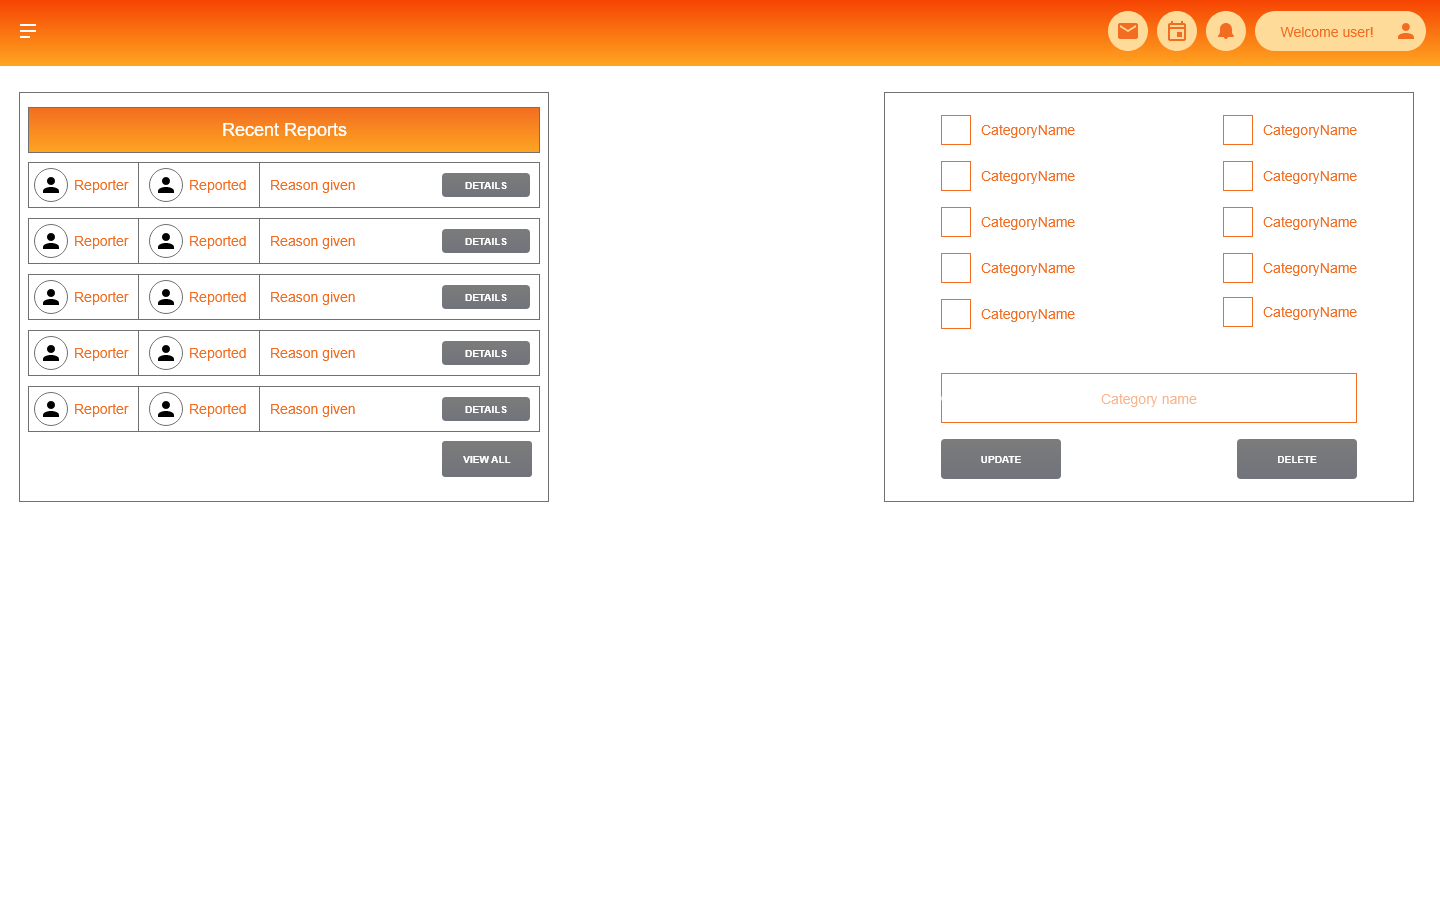
\includegraphics[width=\linewidth]{/prototypes/admin-dashboard.png}
     \caption{Shows the admin dashboard for admins that are logged into the system}
     \label{fig:admin-dashboard}
 \end{figure}
The admin dashboard gives the admin an overview of the recently reported tutors and the different categories. 
The admin needs to see tutor reports since they are the ones that will handle them and decide if a tutor should be banned. 
Admins are also in charge of the different teaching categories, and therefore, they need to have an overview of the current ones and also be able to add new categories.
We also have a top bar that is used on every page for when the user is logged in. It shows a couple of different icons where the user can go to the inbox, the calendar, or the user's own page. 
It will also show notifications for when different events related to the user happen in the system. 
On the far left side of the top bar, we will place a logo, which will lead to the landing page.
\begin{figure}[H]
   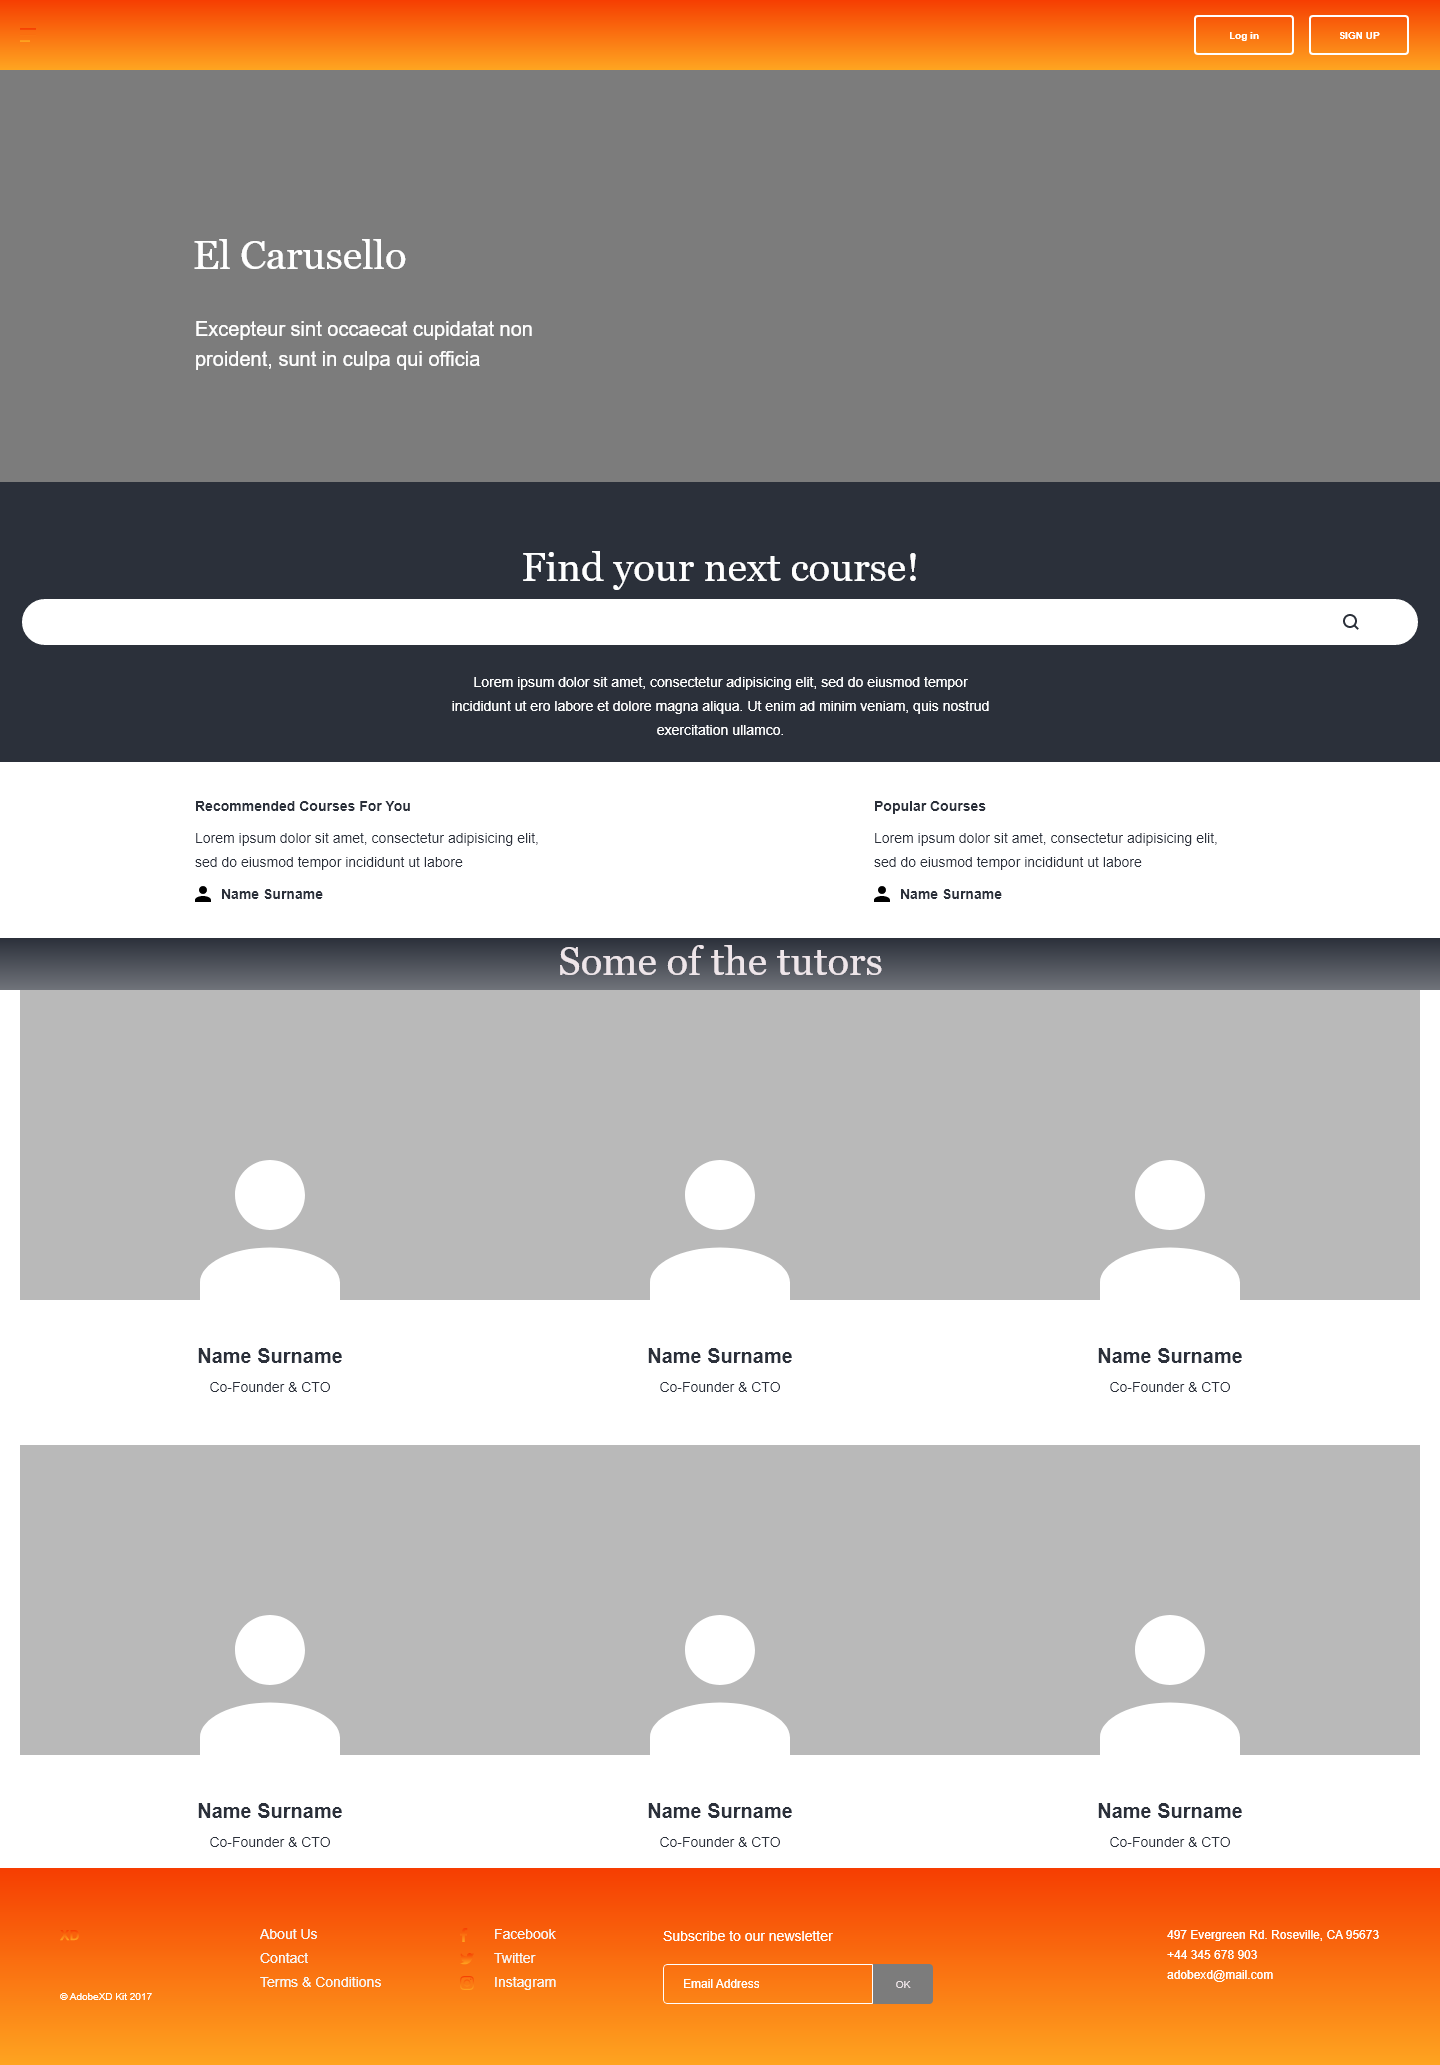
\includegraphics[width=\linewidth, scale=0.5]{/prototypes/landing-page.png}
    \caption{The landing page for the system}
    \label{fig:landing-page}
\end{figure}
The landing page is the first page that the users of the system will see, and thus it is important that this page shows some interesting content. 
This page can be accessed both with and without being logged in. 
We have a top bar that changes depending on if the user is logged in or not. 
At the top of the landing page, we will have a carousel that shows some interesting images.
Underneath, we have included a search functionality to find a course or a specific tutor. 
The user should be able to search for both tutors and courses. 
Finally, there will be some recommendations for the user, which will suggest specific tutors based on their profile information and previously taken courses.

 \begin{figure}[H]
    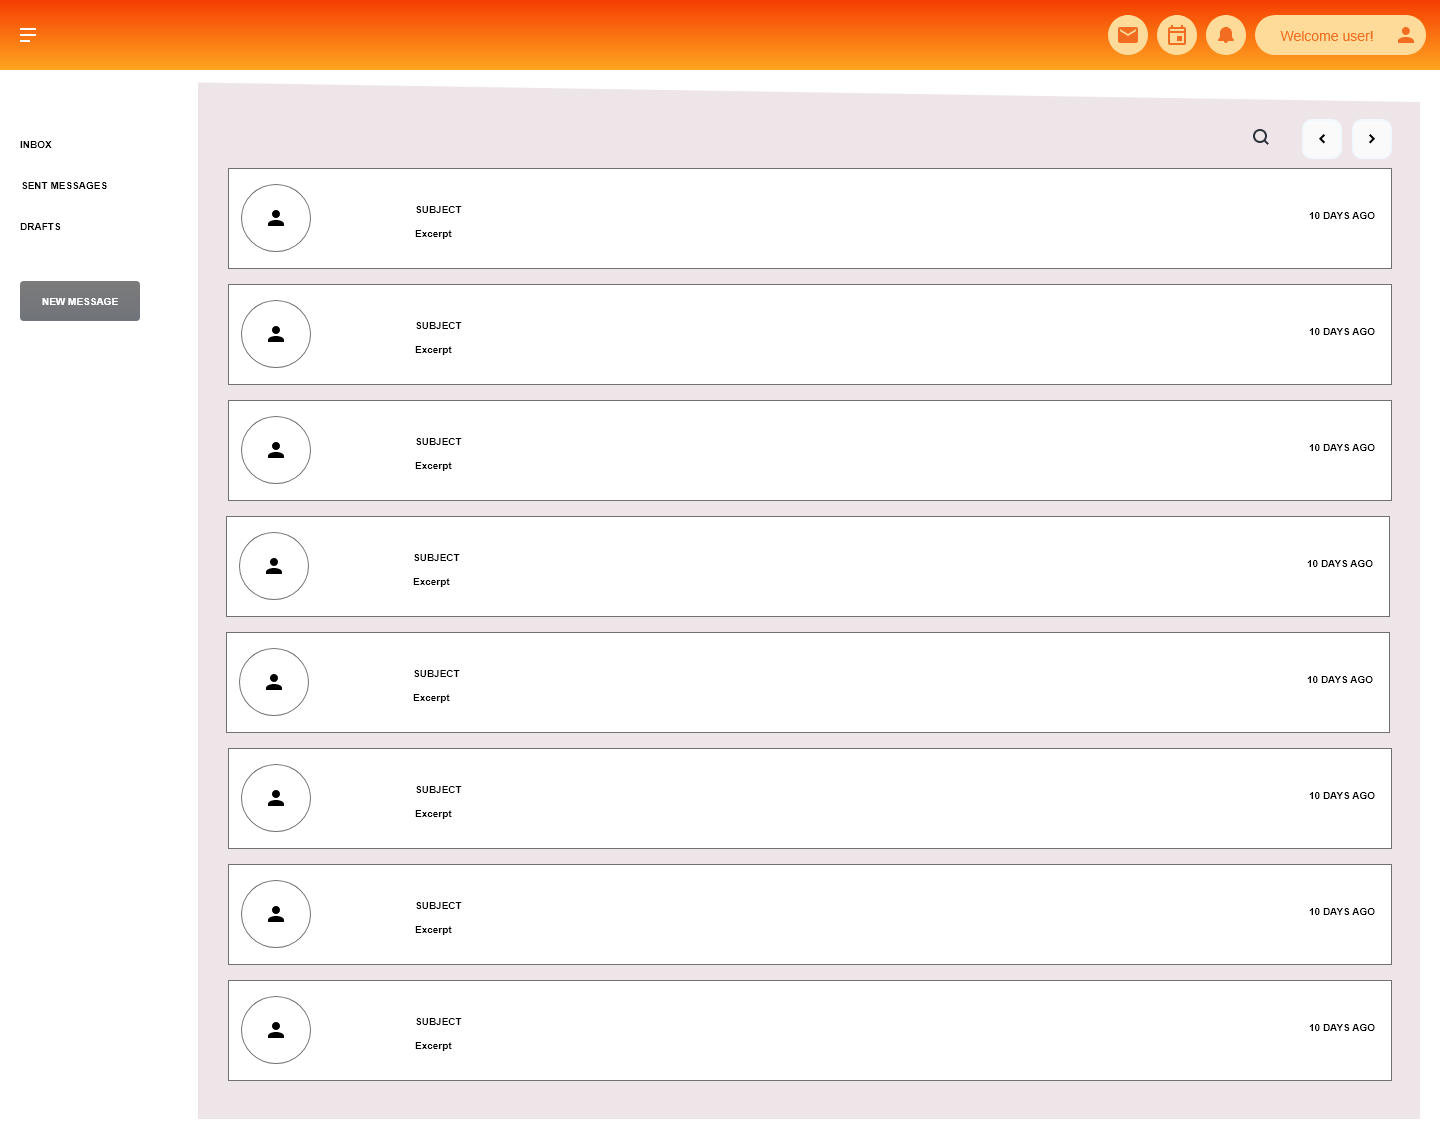
\includegraphics[width=\linewidth]{/prototypes/inbox.png}
     \caption{The inbox for the messaging component in the system}
     \label{fig:inbox}
 \end{figure}
When the user clicks the message icon in the top bar they will be redirected to the inbox page. Here they can view their recent messages. 
We considered including a search functionality to find specific messages but ultimately did not add it to the prototypes. 
The most recently received messages should be shown on the top of the list, so they are easy to find. 
When a message is received, the topbar should also show a notification for this. 
There should also be an indicator that shows if the user has unread messages. 
The user can click a button on the left side of the page to start writing a new message. 


 \begin{figure}[H]
    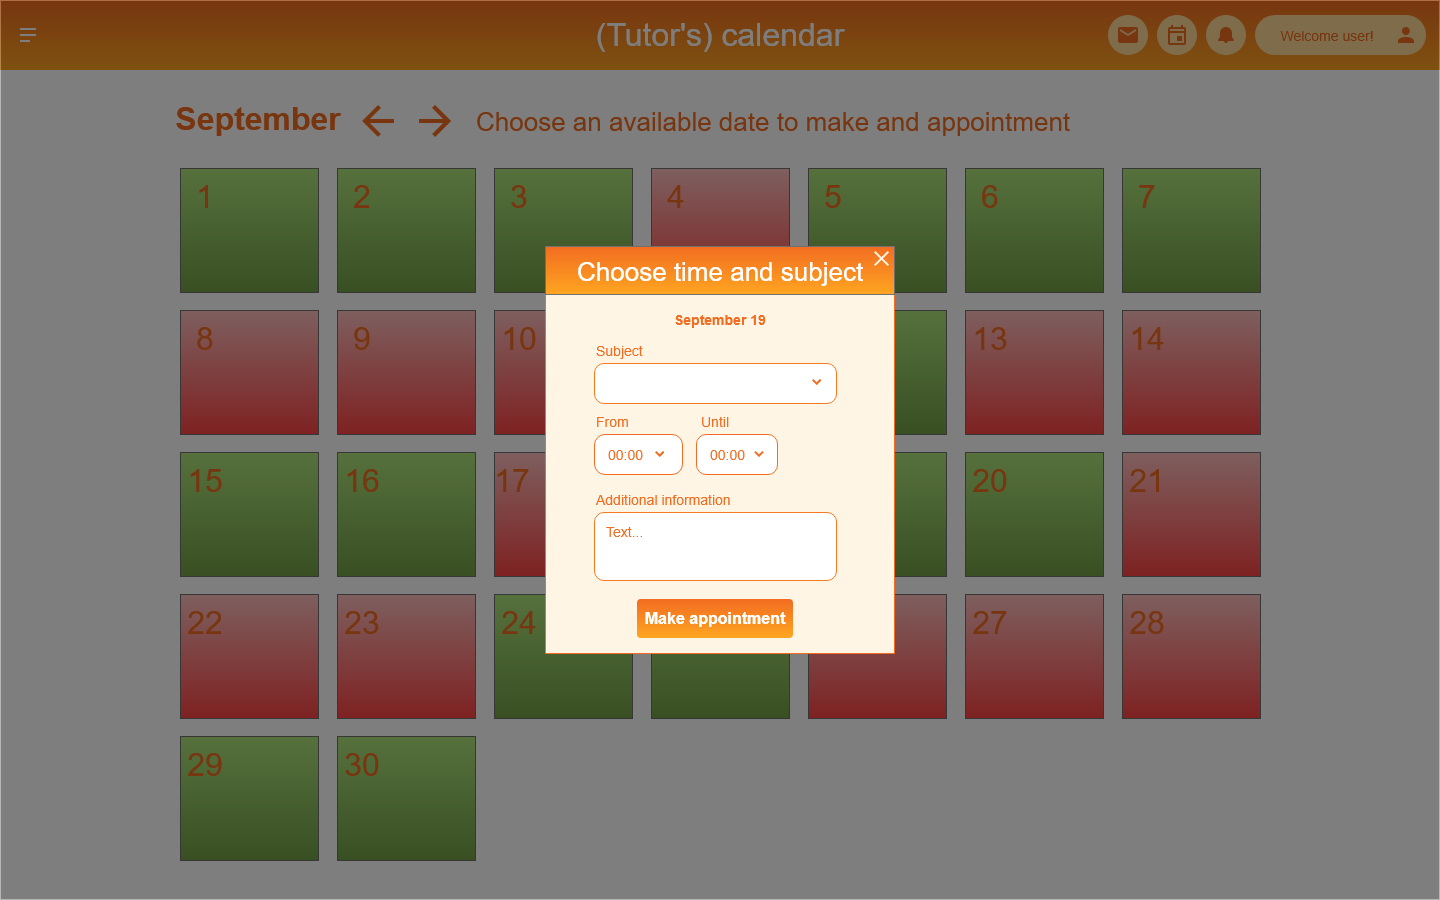
\includegraphics[width=\linewidth]{/prototypes/make-appointment.png}
     \caption{Page that shows a tutor's calendar where the student can request an appointment}
     \label{fig:make-appointment}
 \end{figure}
 This page is the tutor's calendar from a student's point of view. 
 The student is able to browse the tutor's calendar and look for a date where the tutor is available, shown as the color green. 
 The student then clicks the desired date, and the popup window will show. 
 Here they can specify the subject they wish to be taught and the timeslot as well as additional information. 
 They can only choose one of the tutors available subjects, and the timeslot should comply with the tutor's availability. 
 The tutor also needs to choose what time they are available prior to this.
 When the student makes the appointment, they will be sent to a payment page, and a request will be sent to the tutor, which they can either accept or deny.
 However, the money will not be withdrawn from the students account until the tutor has approved the appointment.

 \begin{figure}[H]
    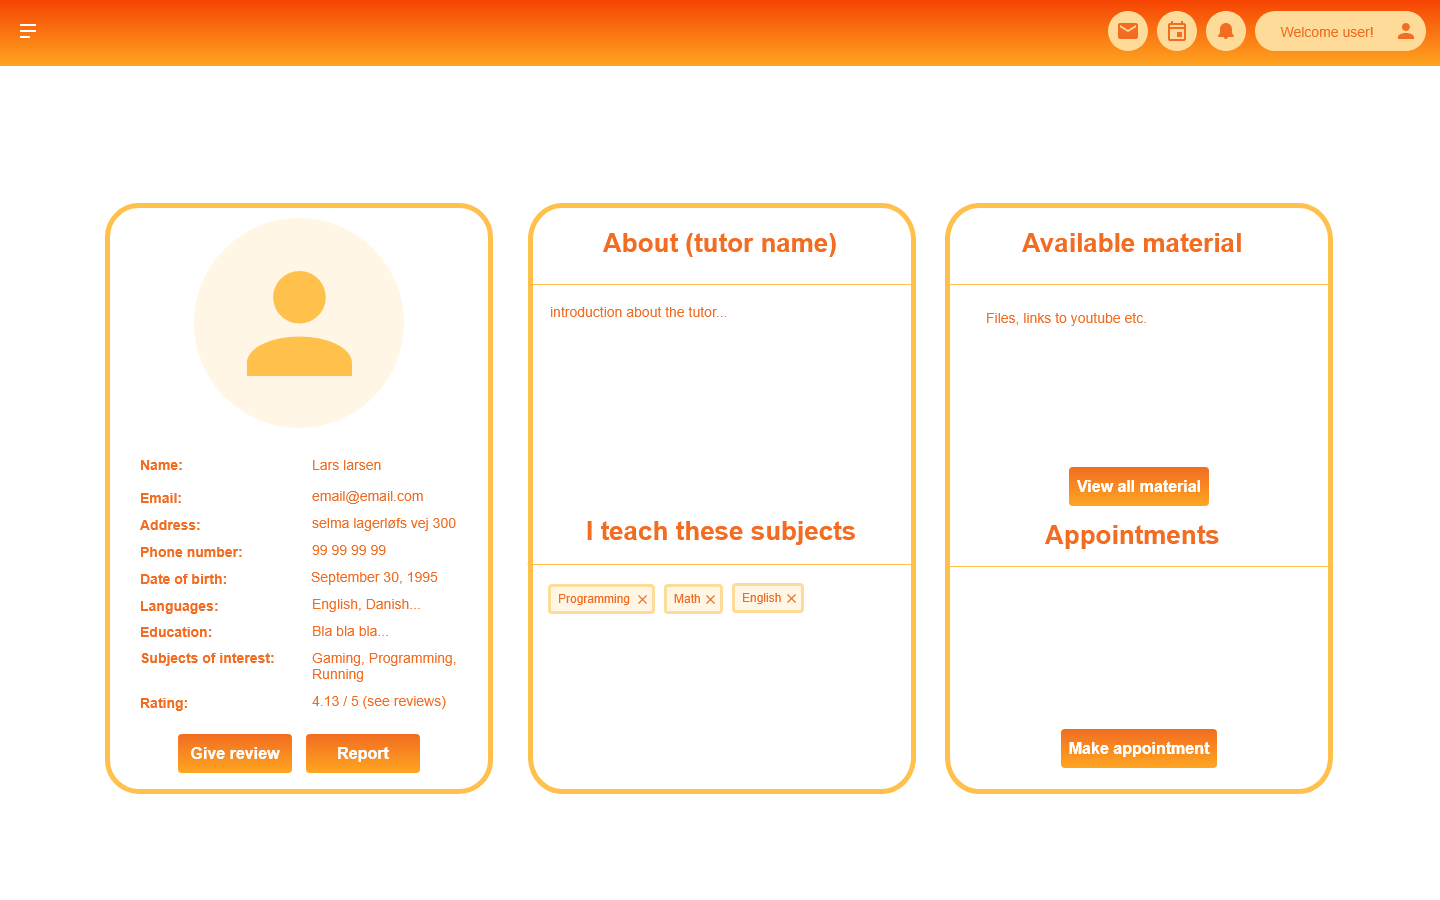
\includegraphics[width=\linewidth]{/prototypes/view-information-on-tutor.png}
     \caption{The page where other users can view information about a specific tutor}
     \label{fig:view-information-on-tutor}
 \end{figure}
This is the page where other users can go and view information about another tutor. 
Much information should be available here so that a user can know if this tutor can be helpful to them.
The page will show basic information on the left side and also show the tutor's rating. 
A user can click \textit{see reviews} to see what other users wrote about the tutor. 
The user viewing the tutor's page can also leave a review of the tutor or report the tutor if they had a bad experience. 
The tutor can display some written information about them in the middle that others can read. 
The middle also shows which subjects the tutor teaches. 
A tutor also has some material connected to their page if they have uploaded any. 
They can make this available to others however they wish, but can also lock it behind payment or only make it available if a student books an appointment with the tutor.
Users can click the \textit{View all material} button to go to the view material page where all the files and links can be found. 
Finally, the user can wish to make an appointment with the tutor. 
By clicking the \textit{Make appointment} button, the user is redirected to the tutor's calendar, where they can find a suitable date for the appointment. 


 \begin{figure}[H]
    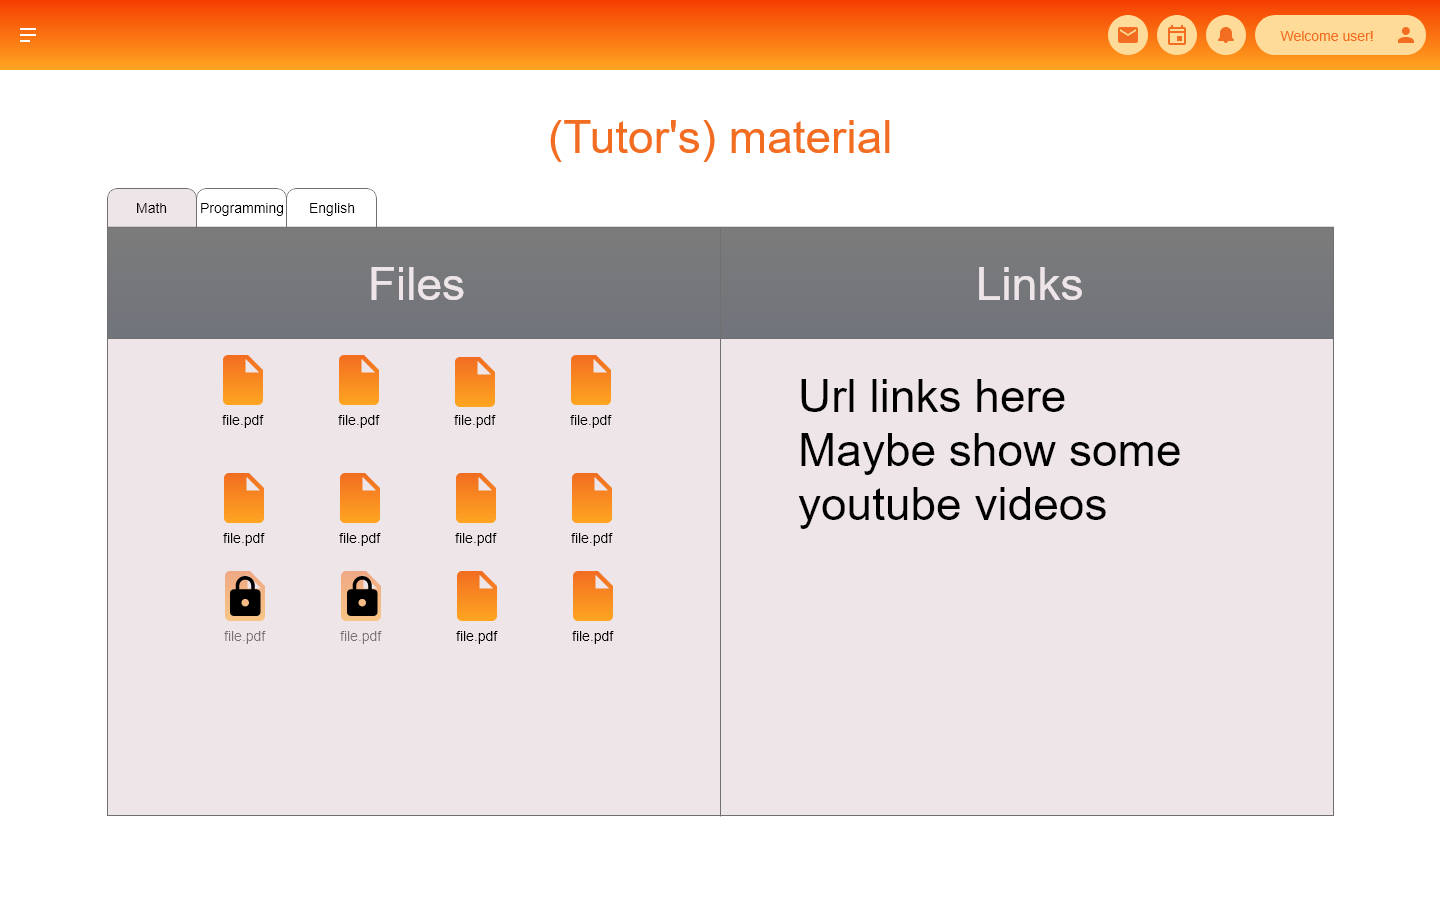
\includegraphics[width=\linewidth]{/prototypes/view-tutor-material.png}
     \caption{The page that shows a tutors available material}
     \label{fig:view-tutor-material}
 \end{figure}
This page shows a specific tutors uploaded material. 
The material is divided into which subject it belongs to make it easier for other users to find the relevant material. 
The material can be any kind of file, or it can be links to useful pages such as some reading material or perhaps a YouTube video. 
When a specific user goes to a tutor's material page, only the material that is accessible to them should be made available. 
All other files should show a lock on top of the file or link to indicate that this item is not available. 
The user can then hover over this item, and it should then tell the user how it can be unlocked. 

\section{Database choice}
The system being developed during this project is heavily focused on scalability, it is therefore important that a database system that can handle a lot of data and which makes scalability easier is chosen.
\\
Furthermore our application is going to handle a variety of data forms. It will store both structured data in the form of user profiles as well as unstructured data such as pictures and videos.
\\
This means that both a relational and non-relational database system could work, making the choice more difficult.
We considered going with a non-relational database, as such database system is often used with our frontend framework React, but since the team has more experience working with relational databases it was decided to go with this kind of database system.
\\
The following databases were looked incorporates
\begin{itemize}
    \item Postgres
    \item MySQL
    \item Oracle
    \item MariaDB
    \item Microsoft SQL Server
\end{itemize}
Postgres is the most advanced opensource relational database \cite{Postgres}.
It is free and is one of the most popular databases being used\cite{databasePopularity}.
It has great documentation and a large active user base.
Furthermore it is not only a relational database but a object-relational database which gives it support for user-defined objects, functions, operators and more.
It also allows storing of Json objects and can therefore be used almost akin to a non-relational database.
Postgres is also ACID compliant, meaning that a database transaction is ensured to be completed even in the event of errors or even power failures.
\\
\\
MySQL is the most popular database used today\cite{databasePopularity}.
It is almost completely open source and has a very active community\cite{MySQL}.
MySQL has also added the functionality to act akin to a non-relational database.
MySQL is not ACID compliant.
\\
\\
Oracle is a commercial database and is quite expensive to obtain\cite{oracle}.
Furthermore you have to pay for extra features.
For these reasons it was decided against using this database.
\\
\\
MariaDB is also a opensource relational-database\cite{MariaDB}.
Just like Postgres it is ACID compliant, can store Json objects and has good documentation.
\\
\\
Microsoft SQL Server is a commercial database system\cite{MSSQLSERVER}.
Like Oracle it means to have access to the full system.
\\
\\
It was decided to use Postgres as the database system.
This was because Postgres also incorporates the ability to handle unstructured data in much the same way a non-relational databases does it, giving us the means to explore that aspect of database design if needed.
The ACID compliance was also deemed important which removed MySQL from the selection process. 
The group also has some experience working with Postgres from an earlier database course which was the last reason to pick it over MariaDB.



\chapter{Implementation}

\section{Supporting multiple languages}
To have a scalable application it is necessary to easily be able to translate the text to different languages.
For this purpose we have used \textit{i18next}, which is an internationalization framework for JavaScript.
Being an internationalization framework means it allows software to be adapted to several languages through localization.
To do this, it makes use of translation files that define the different translations, known as localization files.
I18next is supported for many different frameworks like React, .NET, Angular and many more \cite{i18next}.
Instead of hardcoding the text on every page, we wrap the export of the component in the function \texttt{withTranslations} which injects the function \texttt{t} into the props of the component.
The translation file used for translating is the one corresponding to the language chosen by the user in the header of the system.  

\begin{lstlisting}[caption={Translated header when registering as a user.}, captionpos=b, label={withTranslationsUserForm}]
import { withTranslation } from "react-i18next";

function UserForm(props){
    const { t, classes } = props;

    return (
        <Container maxWidth="sm">
            <div className={classes.paper}>
                <Typography align="center" variant="h4">
                    {t('registerasauser')}
                </Typography>
            ...
    );
}

export default withTranslation()(withStyles(styles)(UserForm))
\end{lstlisting}
\noindent
The translation of the the title on the register page can be seen in \autoref{withTranslationsUserForm}.
The \texttt{withTranslation()} function injects the function t into the props of the \texttt{UserForm} component.
When called, the function t will look up the passed key in the translation files to find the correct translation for \texttt{registerasauser}. 
A screenshot of a snippet of the files can be seen on \autoref{fig:translationfiles}.
\begin{figure}
    \centering
    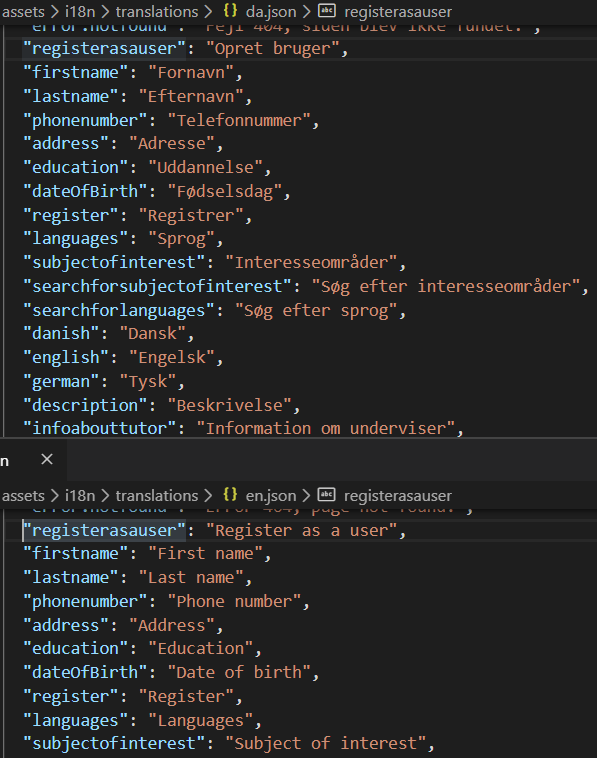
\includegraphics[scale=0.5]{figures/translationexample.PNG}
    \caption{The Danish and English translation files}
    \label{fig:translationfiles}
\end{figure}
\noindent
To add an additional language a new translation file needs to be created.
All the lines that are present in the other files then need to be translated to the desired language. 
It is not necessary to refactor any code to add additional languages.

\section{Structure of the system}
- Something about how we split into API and front end and why. 
- Maybe a refresher about the technologies we use
\section{Structure of API}
This section will describe how how we have implemented and structured the API which is used as a link to the database.

\subsection{Controllers, middlewares, services and routes}
% Controllers, middlewares, services, routes
Something about how the API is split into controllers, middlewares, services and routes.
Talk a bit about each of them and why they are important.

The API is split into controllers so that endpoints that are related to the same entities are in the same controller. 
For example, the \texttt{authController} is responsible for endpoints such as logging in, registering a new user or changing a users password.



\subsection{API responses}
Something about HTTP responses and what to respond.
Maybe briefly mention REST?

\subsection{TypeORM}
With TypeORM we can define entity classes which corresponds to the tables we want to create in the database.
These entities are created as classes with attributes which we can put constraints on such as not allowing an attribute to be null. 
We can also define relationships between entities such as many-to-many and many-to-one.
Objects can be created using the entity classes. 
These objects can be saved to the database or extracted data can be assigned to the objects and then be returned in a HTTP response. 
Typeorm also provides repositories for each entity to allow for easy creation of queries to the database

Something about using TypeORM and why it is nice, so we do not have to make an ORM ourselves, or manually write the queries.

\subsection{Error handling}
Something about logging.

\section{Front end structure}
This chapter focuses on the implementation of the front end in React.
Some basic features within React were previously described in \autoref{sec:intro-to-react}.

\subsection{States}
For many of our pages we use states to store a component's dynamic data. 
An example of this is the edit service page. 
The constructor for this page is seen on \autoref{EditService-state}.
The constructor takes a variable called props as an argument, props contains all of the arguments that the component received when it was instantiated. 
Within the constructor \texttt{super(props)} is called.
This needs to be done to be able to use \texttt{this.props} to access the props anywhere in the component.
Dynamic variables that will be used on the page are initialized in \texttt{this.state}. 
However, if another variable is needed, it can be added to the state at any time as the state is dynamic.\\\\
Variables in the state can be changed by calling the react hook \texttt{this.setState()} and this will automatically trigger a new rendering of the component and all of its children.
For example, it is easy to validate text fields and send an error message if the text input is invalid.  
After the state declarations, we bind the functions to the component instance using the \texttt{.bind(this)} function.
This has to be done if the function uses \texttt{this.setState} to change the state of the component.
Generally it needs to be done for all functions that need to access React hooks through \texttt{this}.
\begin{lstlisting}[caption={Constructor and state for edit service}, captionpos=b, label={EditService-state}]
class EditService extends React.Component {
    constructor(props) {
        super(props);
    
        this.state = {
            service: null,
            categories: [],
            chosenCategoryNames: [],
            redirectService: false,
            redirectOwnUser: false,
            openAlert: false
        };
            
        this.handleOnChange = this.handleOnChange.bind(this);
        this.handleOnChangeCategories = this.handleOnChangeCategories.bind(this);
        this.submit = this.submit.bind(this);
        this.deleteService = this.deleteService.bind(this);
        this.handleClickCancel = this.handleClickCancel.bind(this);
        this.handleClickDelete = this.handleClickDelete.bind(this);
        this.handleClickOpen = this.handleClickOpen.bind(this);
    }
    (*@\centerline{\raisebox{-1pt}[0pt][0pt]{$\vdots$}}@*)
\end{lstlisting}

\subsection{Services}
Services are used to send or retrieve data from the API. 
\autoref{get-by-id} shows an example or retrieving a user by their id from the database.
The \texttt{requestOptions} used as a parameter defines the type of method you use.\\
For \texttt{'POST'} methods the \texttt{requestOptions} will contain the data to send to the API as the body of the request.
For many requests it is necessary for the user to be logged in, which is defined in the header of the request through the function \texttt{authHeader()}, which checks if the user is logged in.\\
The fetch is then called with the URL link and the response is handled with the \texttt{handleResponse} function. 
This is a function that checks for errors in the response, and ensures that the user requesting the response has the proper privileges to access it.

\begin{lstlisting}[caption={Function to get a user by ID.}, captionpos=b, label={get-by-id}]
function getById(id) {
	const requestOptions = { method: 'GET', headers: authHeader() };
	return fetch(
        `http://${process.env.REACT_APP_API_URI}:
           ${process.env.REACT_APP_API_PORT}/api/users/${id}`,
		requestOptions
	)
		.then(handleResponse)
		.then(data => {
			return JSON.parse(data);
		});
}
\end{lstlisting}

\subsection{Components}
There are two types of components. 
The first one is a stateful component, also called a container.
These are typically class components and have a state.
They often contain some kind of logic and some conditional rendering dependent on the current state.
The second is a presentational component.
These are most often stateless and are called presentational since all they should do is output UI elements \cite{Vumbula-react}.

\begin{figure}[H]
    \centering
    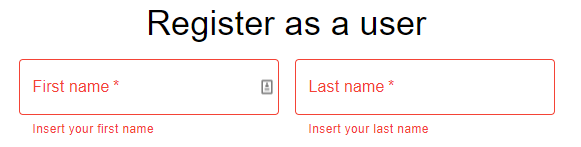
\includegraphics[scale=0.5]{figures/create-user-error.png}
    \caption{Error message when creating a user}
    \label{fig:create-user-error}
\end{figure}
\noindent
The container for the create user page can be seen on \autoref{create-user}.
The \texttt{CreateUser} class only contains the state, some functions and a \texttt{render()}.
Within the state object of \texttt{CreateUser}, there is an object called \texttt{firstName}, which contains a \texttt{firstName} string and a \texttt{firstNameValid} boolean to indicate if \texttt{firstName} is valid.
It is initialized as true, so that the error messages are not visible when entering the page.
When they press the submit button, the \texttt{handleSubmit} function will be called, which checks if the values are valid.
If the values are invalid, the booleans in the state will be updated. 
If these are set to false, an error message will be shown as can be seen in \autoref{fig:create-user-error}.

The presentational component \texttt{UserForm} is rendered in the \texttt{render()} function. 
\begin{lstlisting}[caption={Component to create user}, captionpos=b, label={create-user}]
export class CreateUser extends Component {
    constructor(props) {
        super(props);
        this.state = {
            firstName: { firstName: '', firstNameValid: true },
            lastName: { lastName: '', lastNameValid: true },
            (*@\centerline{\raisebox{-1pt}[0pt][0pt]{$\vdots$}}@*)
        };
        this.handleChange = this.handleChange.bind(this);
        this.handleSubmit = this.handleSubmit.bind(this);
    }
    (*@\centerline{\raisebox{-1pt}[0pt][0pt]{$\vdots$}}@*)
    render() {
        return (
            <UserForm
                firstName={this.state.firstName}
                lastName={this.state.lastName}
                (*@\centerline{\raisebox{-1pt}[0pt][0pt]{$\vdots$}}@*)
            />
        );
    }
\end{lstlisting}
The implementation of \texttt{UserForm} can be seen on \autoref{user-form}.
This presentational component is stateless and uses the props that were passed to the \texttt{UserForm} component when it was instantiated in the \autoref{create-user} container.
Within the \texttt{TextField} it checks through props if the first name is valid. 
If it is not valid an error will be shown, and the \texttt{helperText} will also be shown.
Whenever the \texttt{TextField} is changed the \texttt{handleChange} is called, and as it changes the state of the parent component the page will be re-rendered.

\begin{lstlisting}[caption={Presentational component for userform}, captionpos=b, label={user-form}]
function UserForm(props) {
    const { t, classes } = props;
    
    return (
        <Container maxWidth="sm">
            <div className={classes.paper}>
                <Typography align="center" variant="h4">
                    {t('registerasauser')}
                </Typography>
                <div className={classes.form}>
                <Grid container spacing={2} direction="row">
                    <Grid item xs={12} sm={6}>
                        <TextField
                            name="firstname"
                            label={t('firstname')}
                            onChange={props.handleChange}
                            error={!props.firstName.firstNameValid}
                            helperText={
                                props.firstName.firstNameValid ? '' : t('typefirstname')
                            }
                        />
                        (*@\centerline{\raisebox{-1pt}[0pt][0pt]{$\vdots$}}@*)
\end{lstlisting}

\subsection{Material-UI}
We have chosen to use the framework \textit{Material-UI}, to ease the implementation of design, and ensure it is of a certain quality.
Material-UI is a collection of React components that are easy to integrate into the project.
If we had to implement everything ourselves we would have to invest a lot of more time into making a good design.
By using Material-UI for the design we also get consistently designed pages.
Some of the most commonly used components in our application are \texttt{TextField}, \texttt{Typography}, \texttt{Grid}, \texttt{Button} or \texttt{MenuItem}.
An example of using Material-UI in the header can be seen on \autoref{material-ui}.
As seen in the begin of the file, we import the different components that are needed.
From line 11 onwards we then use them to create the design.
The header can be seen on \autoref{fig:header}.
In \autoref{material-ui} we implement parts of the header, more specifically the log in icon in the right side.
If the button is pressed, the user is redirected to the login page.
\begin{lstlisting}[caption={Use of material-ui in the header}, captionpos=b, label={material-ui}]
import {
    List,
    ListItem,
    ListItemIcon,
    ListItemText
} from '@material-ui/core';
import {
	ExitToApp
} from '@material-ui/icons';
(*@\centerline{\raisebox{-1pt}[0pt][0pt]{$\vdots$}}@*)
<List>
    <ListItem button component={Link} to="/login" key="LoginCircle" name="login">
        <ListItemText primary="Login" />
        <ListItemIcon>
            <ExitToApp fontSize="large" />
        </ListItemIcon>
    </ListItem>
(*@\centerline{\raisebox{-1pt}[0pt][0pt]{$\vdots$}}@*)
\end{lstlisting}


\begin{figure}[H]
    
\includegraphics[width=\linewidth]{figures/header.png}
    \caption{The header for the application}
    \label{fig:header}
\end{figure}

\section{Supporting multiple languages}
To have a scalable application it is necessary to easily be able to translate the text to different languages.
For this purpose we have used \textit{i18next}, which is an internationalization framework for JavaScript.
Being an internationalization framework means it allows software to be adapted to several languages through localization.
To do this, it makes use of translation files that define the different translations, known as localization files.
I18next is supported for many different frameworks like React, .NET, Angular and many more \cite{i18next}.
Instead of hardcoding the text on every page, we wrap the export of the component in the function \texttt{withTranslations} which injects the function \texttt{t} into the props of the component.
The translation file used for translating is the one corresponding to the language chosen by the user in the header of the system.  

\begin{lstlisting}[caption={Translated header when registering as a user.}, captionpos=b, label={withTranslationsUserForm}]
import { withTranslation } from "react-i18next";

function UserForm(props){
    const { t, classes } = props;

    return (
        <Container maxWidth="sm">
            <div className={classes.paper}>
                <Typography align="center" variant="h4">
                    {t('registerasauser')}
                </Typography>
            ...
    );
}

export default withTranslation()(withStyles(styles)(UserForm))
\end{lstlisting}
\noindent
The translation of the the title on the register page can be seen in \autoref{withTranslationsUserForm}.
The \texttt{withTranslation()} function injects the function t into the props of the \texttt{UserForm} component.
When called, the function t will look up the passed key in the translation files to find the correct translation for \texttt{registerasauser}. 
A screenshot of a snippet of the files can be seen on \autoref{fig:translationfiles}.
\begin{figure}
    \centering
    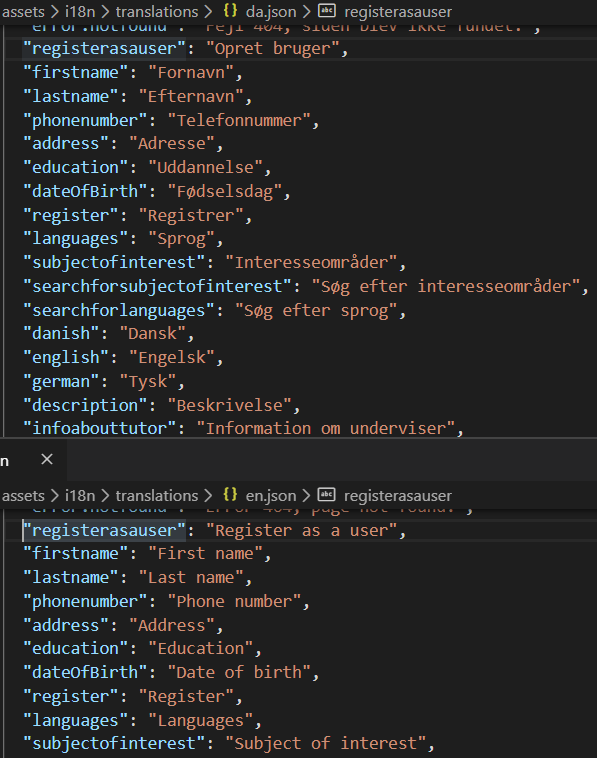
\includegraphics[scale=0.5]{figures/translationexample.PNG}
    \caption{The Danish and English translation files}
    \label{fig:translationfiles}
\end{figure}
\noindent
To add an additional language a new translation file needs to be created.
All the lines that are present in the other files then need to be translated to the desired language. 
It is not necessary to refactor any code to add additional languages.

\section{Recommender system}\label{Recommender-system}
It would be beneficial to provide a way for users to see relevant, interesting services for their preferences, in order to make the system more usable.
To accomplish this, a recommender system can be used.
The following section will detail different ways of implementing such a system, which one we chose and why, and finally our implementation of a recommender system.

\subsection{The purpose of a recommender system}
When searching for something new, information overload can occur.
Many different sources can provide information that might not be relevant.
If a new user interacts with this system, seeking to find a new subject in which to attain knowledge, this user could potentially be presented with an overwhelming amount of services, depending on how many tutors have made these available.
Another issue that might arise is that not all of the services will be relevant for the new user, serving only to clog the list of services. 
This leads to information overload, where the retrieved information in the form of services is not what the user needs, and not enough of the correctly relevant information is returned.
Recommender systems are used to remedy these issues.
They help match users with relevant items, in this case services, to ease the information overload.
This generates value for both the user and the tutor, in that users are matched with what they have a predilection for, and tutors can reach more prospective students.
We discuss two methods of creating a recommender, \textit{content-based filtering} and \textit{collaborative filtering}.

\subsection{Content-based filtering}\label{content-based-filtering}
Content-based recommender systems recommend an item to a user based upon a description of the item and a profile of the user's interests \cite{ContentBasedFiltering}.
A common scenario for web applications is that they present a list of items to a user, and the user then selects among these to receive more details. 
An item in such a scenario would have a representation dependent on the implementation, which could be used to analyze items of particular interest for a user.
Items are often stored in databases, creating structured data with each entry having the same set of attributes. 
This lends itself well to learning a user profile through different machine learning algorithms.
Examples of a basic representation of items and users are shown in Tables \ref{tbl:content-item} and \ref{tbl:content-user}.
As shown, users and items are represented by the same set of attributes.
\begin{table}[H]
    \centering
    \begin{tabular}{|l|l|l|l|l|}
    \hline
    Title                                         & Genre    & Author        & Price & Type      \\ \hline
    Blue Moon                                     & Thriller & Lee Child     & 10    & Hardcover \\ \hline
    Norse Mythology                               & Fantasy  & Neil Gaiman   & 6     & Paperback \\ \hline
    Normandy ‘44: D-Day and the Battle for France & History  & James Holland & 14    & Hardcover \\ \hline
    \end{tabular}
    \caption{This figure shows a possible representation of a few items for content-based filtering.}
    \label{tbl:content-item}
\end{table}
\begin{table}[H]
    \centering
    \begin{tabular}{|l|l|l|l|l|}
    \hline
    Title                                         & Genre    & Author        & Price & Type      \\ \hline
    ... & Fantasy  & George R. R. Martin, J.K. Rowling & 5    & Paperback \\\hline
    \end{tabular}
    \caption{This figure shows a possible representation of a user.}
    \label{tbl:content-user}
\end{table}

\todo{table er næsten for langt til siden}
\noindent
The basic idea for content-based filtering is then to compute the similarity of an unseen item with the user profile, and suggest the items with attributes that are most similar to those in the user profile..
Unstructured data, such as text fields with no restriction, create complications when creating a user profile, as relationships between the values on an attribute for different items for a specific user can be found, but an unrestricted text will generally be unique \cite{ContentBasedFiltering}. 
If a user liked different restaurants based on the same cuisine, it could be indicated that this user would be likely to like other restaurants focused in the same cuisine as well, but a text review would not necessarily give this information.
Many domains can be represented by semi-structured data where issues arising from certain types of unstructured data, such as text fields, are converted to a structured representation \cite{ContentBasedFiltering}.
A user profile shows the preferences of the user, and consists mainly of two types of information:
\begin{itemize}
    \item A description of the types of items that interest the user
    \item A history of the user's interactions with the recommender system, such as storing the items that a user has viewed and information related to the interaction, such as if the user purchased the item.
\end{itemize}
Historical data of interactions can be used to filter out already purchased items, display recently visited items or as training data.
Creating a model of a user's preferences is then done through a form of classification learning, in which training data is divided into categories, an example being the binary categories \textit{Items the user likes} and \textit{items the user dislikes} \cite{ContentBasedFiltering}.
These algorithms learn a function that model's a users interests, and given a new item and the user model, this function predicts whether or not the user is interested in the item through a probability or a numeric value by analyzing the item representation and user profile.
Popular learning approaches for content-based filtering are \textit{naïve Bayes}, \textit{nearest neighbor methods} or \textit{linear classifiers}.

\subsection{Collaborative filtering}
Collaborative filtering differs from content-based filtering in that it focuses on matching users and items through the opinions of other people.
Collaborative filtering is based on word-of-mouth recommendations.
A person might have friends that recommend different things, and will eventually learn which of these friends has tastes that most align with their own, and thus which recommendation to value the most.
Collaborative filtering extends this concept \cite{CollaborativeFiltering}.
Collaborative filtering makes use of ratings.
These could be ratings between 1-5 or 1-10, for example, or simply binary ratings.
A rating is an association of two things, a user and a value.
A matrix of ratings can then be constructed, as shown in \autoref{tbl:collaborative-example}.
The empty entries indicate that the user has not rated the item, and are what the system should be able to predict.
\begin{table}[H]
    \centering
    \begin{tabular}{|l|l|l|l|l|}
    \hline
           & Item1 & Item2 & Item3 & Item4 \\ \hline
    Peter  & 3     &       & 5     &       \\ \hline
    Amy    & 4     & 2     &       & 3     \\ \hline
    Lars   &       & 5     & 3     & 2     \\ \hline
    Martin & 1     &       & 2     & 4     \\ \hline
    \end{tabular}
    \caption{This figure shows an example of a ratings matrix, with ratings from 1 to 5. An empty entry indicates that the user has not rated the item.}
    \label{tbl:collaborative-example}
\end{table}
\noindent
Domains with certain properties lend themselves to collaborative filtering. 
These are \textit{data distribution}, \textit{underlying meaning} and \textit{data persistence} \cite{CollaborativeFiltering}.
Data distribution encompasses domains in which there are many items, many ratings per item, more users rating that items to be recommended and users rate multiple items.
Underlying meaning encompasses domains in which users can have tastes in common, evaluation of an item cannot be done objectively and items are homogenous.
Data persistence encompasses domains in which items persist and taste persists, meaning the tastes of the users do not change rapidly.
Collaborative filtering usually makes use of \texttt{k nearest neighbor} algorithms based on users or items, or latent factor models to create predictions.
The user-based nearest neighbor approach focuses on finding users with similar tastes from which to predict a given user's rating, whereas the item-based approach focuses on finding items similar to a given item, and then taking the user's ratings for those similar items to predict a rating for an unrated item.
The latent factor approach focuses on splitting the rating matrix into separate matrices through matrix factorization to simulate communities, and creating predictions from these.


\subsection{Pros and cons}\label{sec:recommender-pros-and-cons}
Content-based filtering and collaborative filtering use different underlying assumptions \cite{CollaborativeFiltering}.
Content-based filtering assumes that items with similar objective features will be rated similarly, whereas collaborative filtering assumes that people with similar tastes rate things similarly, and that customers who had similar tastes in the past will have similar tastes in the future.
The assumption that collaborative filtering employs, that users will have similar taste in the future, is quite strong and cannot be guaranteed, as tastes are likely to change over time.
Content-based filtering can predict relevance for items without ratings by looking at similar items, whereas collaborative filtering requires ratings for an item to create predictions.
This means content-based filtering is especially useful for items that change a lot, but it needs content to analyze.
For domains where content is scarce, such as for a system in which users rate movies since a small amount of users will actually leave a rating, collaborative filtering has an edge since it does not require content.
Content-based techniques can have problems with new users, as there is a ramp-up phase when learning a model of the user's interests.
To do so, it needs explicit or implicit feedback, and there is no guarantee that the user leaves explicit feedback such as a rating, and implicit feedback from a user's behavior can be imprecise.
Since collaborative filtering requires ratings for an item to create predictions it has issues with cold starts.
If a new item is added, it will not have any initial ratings from users, which means creating a prediction becomes different as it has nothing from which to base the prediction.
Collaborative filtering methods making use of \texttt{k nearest neighbor} methods can have scalability issues, as the rating matrix can grow to be very large as more users join the service or more items are added.
This is a problem that latent factor models alleviate, as they reduce the size of the rating matrix through splits.
Content-based and collaborative filtering are not mutually exclusive, and both can be used in a complementary fashion to avoid some of the issues that arise when using just one.
\begin{table}[]
    \begin{tabular}{|p{.2\textwidth}|p{.4\textwidth}|p{.4\textwidth}|}
    \hline
                    & Content-based                                              & Collaborative                                                             \\ \hline
    Assumptions     & Items with similar features are rated similarly            & People with similar taste rate items similarly, taste will not change     \\ \hline
    Requirements    & Does not need ratings, but content to analyze              & Needs ratings but not content                                             \\ \hline
    Item changes    & Deals well with changing items by looking at similar items & Does not deal well with new items, as it needs initial ratings on an item \\ \hline
    Start-up issues & New users can have large ramp-up                           & Cold starts with new items                                                \\ \hline
    \end{tabular}
    \caption{A comparison of the pros and cons}
    \label{tab:recprosandcons}
    \end{table}

\subsection{Our choice}
Ideally, a combination of both collaborative and content-based filtering is ideal.
However, for this project implementing such a combination was not feasible, and we had to focus on one type of recommender system.
The reason it was not feasible was due to the recommender system being based on knowledge acquired from one of the semester courses, and such systems were only detailed towards the end of the semester, leading to a lack of time to create a combined solution.
The system has a simple rating system in which users rate a service on a numerical scale of one to five.
It is assumed that services will be rated by a small subset of users, since not all users will participate in all services, and not all who participate in a given service will leave a rating of it.
This means the domain will have content that is scarce.
It is also assumed that services will not change a lot.
If a service is based around swimming, we do not expect that it will quickly be changed to feature another subject matter, but rather a new service be added by the same tutor with the new subject matter.
As such, the better choice would be collaborative filtering, as the domain lends itself more to this type of system.
In terms of which approach to collaborative filtering to use, the added scalability of a latent factor model provides it an edge for this system as it focuses on scalability.

\subsection{Collaborative filtering through a latent factor model}
The latent factor model approach to collaborative filtering is an approach that tries to explain the ratings by characterizing both items and users on a number of factors.
This number of factors is usually 20-100 \cite{MatrixFactorization}. 
The factors are thought of as measures that measure dimensions.
For example, for movies, the factors could be thought of as measuring obvious dimensions such as amount of action, less well-defined dimensions such as character development or uninterpretable dimensions \cite{MatrixFactorization}.
\autoref{fig:latent-factor} shows an example of a latent factor approach with two dimensions.
It shows an example of how users and movies could be characterized based on the dimensions.
A user's predicted rating for a movie would then be equal to the dot product of the user's and movie's location on the graph, for example, user 5 would be expected to like movie 1, think movie 4 is average and dislike movie 2.
\begin{figure}[H]
    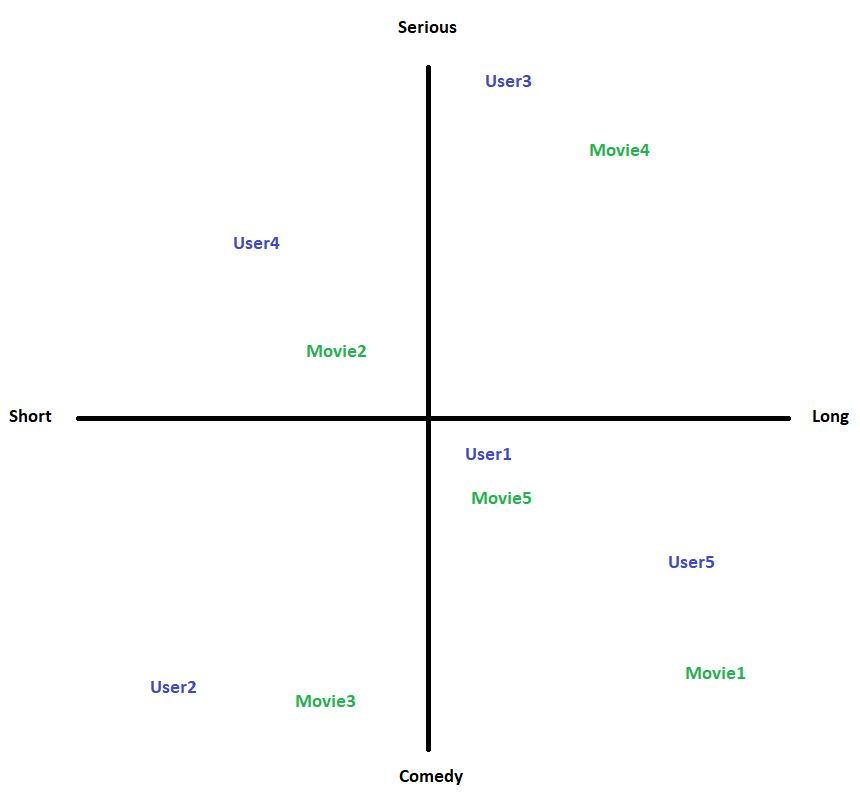
\includegraphics[width=\linewidth]{/recommender/latentfactor.JPG}
     \caption{A simplified illustration of a latent factor approach.}
     \label{fig:latent-factor}
 \end{figure}
 \noindent
A popular method of approaching a latent factor model is through matrix factorization.
Matrix factorization aims to characterize items and users by vectors of factors, and a recommendation would be found by a similarity between these.

\subsubsection{Matrix factorization}
Matrix factorization map users and items to a latent factor space of dimensionality \textit{f} \cite{MatrixFactorization}. 
This is achieved by taking the ratings matrix and splitting it into two matrices of the following dimensions, where $N_{i}$ is the number of items, $N_{u}$ is the number of users and $f$ is the number of factors:
\begin{equation}
    N_{i} \times f
\end{equation} 
\begin{equation}
    f \times N_{u}
\end{equation}
This results in each item \textit{i} and each user \textit{u} being associated with vectors: 
\begin{equation}
    q_{i} \epsilon \mathbb{R}^f
\end{equation}
\begin{equation}
    p_{u} \epsilon \mathbb{R}^f
\end{equation}
For a given item, the elements of $q_{i}$ measures the extent to which an item possesses the factors, and the elements of $p_{u}$ measures the interest of a user in items that are highly valued on the corresponding factor \cite{MatrixFactorization}.
The dot product of these two vectors then describes the user's overall interest in the item, leading to an estimate of:
\begin{figure}[H]
    \centering
    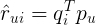
\includegraphics[]{/recommender/predictrating.png}
     \caption{How a prediction for a rating is calculated}
     \label{fig:predictrating}
 \end{figure}
 \noindent
To learn the factor vectors $p_{u}$ and $q_{i}$ used for the equation in \autoref{fig:predictrating}, the recommender system minimizes the squared error of the set of known ratings, that is, the entries in the ratings matrix that have a value:
 \begin{figure}[H]
    \centering
    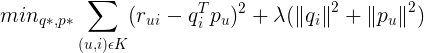
\includegraphics{/recommender/minimizesquarederror.png}
     \caption{How to calculate the squared error once predictions have been made}
     \label{fig:minimizesquarederror}
 \end{figure}
 \noindent
 In \autoref{fig:minimizesquarederror}, $K$ is the set of $(u, i)$ pairs for which the rating $r_{ui}$ is known.
 The system learns by fitting previously observed data, but to avoid overfitting when predicting future ratings, it regularizes the learned parameters.
 This regularization is found on the right side of the $+$ operator of the equation, where $\lambda$ is an arbitrary constant that controls the extent of the regularization.
 Stochastic gradient descent is one approach of minimizing the above equation.
 The algorithm will, in this approach, loop through all data in the training set, which is the known ratings.
 For each case, the system predicts a rating, and then computes the prediction error with the equation defined in \autoref{fig:calculatingerror}:
 \begin{figure}[H]
    \centering
    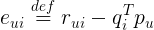
\includegraphics[]{/recommender/calculatingerror.png}
     \caption{The equation for calculating the error of a prediction when the actual value is known}
     \label{fig:calculatingerror}
 \end{figure}
 \noindent
 After the error has been calculated, the algorithm modifies the parameters through the updates rules shown in Figures \ref{fig:updatingq} and \ref{fig:updatingp}:
 \begin{figure}[H]
    \centering
    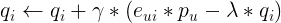
\includegraphics[]{/recommender/updatingq.png}
     \caption{The rule for updating the value of $q$}
     \label{fig:updatingq}
 \end{figure}
 \noindent
 
 \begin{figure}[H]
    \centering
    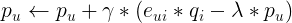
\includegraphics[]{/recommender/updatingp.png}
     \caption{The rule for updating the value of $p$}
     \label{fig:updatingp}
 \end{figure}
 \noindent
 For the update rules, $\gamma$ is the magnitude to which the parameters are modified, and is arbitrary.
 The calculations are performed until the squared error reaches a sufficiently small value, or a max number of iterations has been performed by the algorithm.
 
\subsection{Our implementation}
In \autoref{lst:recomstart} we initially make use of our other services to get the required data to predict ratings.
To perform the calculations we need all users, all services and all ratings currently in the database.
We then initialize the necessary matrices.
These are matrices with dimensions of respectively $users \times servcices$, $users \times factors$, $factors \times services$. 
For the ratings matrix which is $users \times services$ we call a function to populate it.
This is done by traversing the matrix, and for each rating in the \texttt{allRatings} variable, we search the ratings matrix for ids corresponding to the service and user ids of that rating.
If found, we insert the rating value into that entry.
\begin{lstlisting}[caption={The start of the recommender}, captionpos=b, label={lst:recomstart}]
export default class Recommender {
    static async calculateRecommendations(): Promise<number[][]> {
        const allUsers = await UserService.getAll();
        const allServices = await ServiceService.getAll();
        const allRatings = await RatingService.getAll();
    
        let userServiceMatrix: number[][] = [];
        let predictedRatings: number[][] = [];
        let userFactorMatrix: number[][] = [];
        let factorServiceMatrix: number[][] = [];

        userServiceMatrix = initUserServiceMatrix(numberOfRows, numberOfCols, allUsers, allServices, userServiceMatrix);

		userServiceMatrix = populateUserServiceMatrix(allRatings, numberOfRows, numberOfCols, userServiceMatrix);
(*@\centerline{\raisebox{-1pt}[0pt][0pt]{$\vdots$}}@*)
\end{lstlisting}
When we initialize both the matrix for users and factors as well as the matrix for factors and services we initialize all entries with random values between 0 and 1.
Initialization is illustrated in \autoref{lst:initUserFactor}.
This is done to ensure we can calculate a predicted rating.
The actual value is arbitrary, but a small value is chosen, as this should make the algorithm arrive at a model faster, compared to initializing with a greater value \cite{FunkMatrixFactorization}.
\begin{lstlisting}[caption={Initializing the user and factor matrix}, captionpos=b, label={lst:initUserFactor}]
function initUserFactorMatrix(numberOfRows: number, numberOfFactors: number, userFactorMatrix: number[][]): number[][] {
    for (let i = 0; i < numberOfRows; i++) {
        userFactorMatrix[i] = []; // Initialize inner array
        for (let j = 0; j < numberOfFactors; j++) {
            userFactorMatrix[i][j] = Math.random();
        }
    }   
    return userFactorMatrix;
}
\end{lstlisting}
\autoref{lst:initUserService} illustrates how we initialize the matrix for users and services.
On the first row we insert the ids of all services, and on the first column we insert all user ids.
This is done to ensure we can get the proper ids for the users and services to recommend.
Then we insert 0 in all entries, and call another function to populate the entries in which there are ratings.
If there is a rating from a user on a given service, we find the entry corresponding to these ids and insert the rating value.
This means we end with a matrix consisting of a row of service ids, a column of user ids, the rating values and 0 for those entries without ratings.
\begin{lstlisting}[caption={Initializing the user and service matrix}, captionpos=b, label={lst:initUserService}]
    export function initUserServiceMatrix(
	numberOfRows: number,
	numberOfCols: number,
	allUsers: User[],
	allServices: Service[],
	userServiceMatrix: number[][],
): number[][] {
	userServiceMatrix[0] = [];
	for (let i = 0; i < numberOfRows; i++) {
		userServiceMatrix[i + 1] = [];
		userServiceMatrix[i + 1][0] = allUsers[i].id;
	}

	for (let i = 0; i < numberOfCols; i++) {
		userServiceMatrix[0][i + 1] = allServices[i].id;
	}

	for (let i = 1; i < numberOfRows + 1; i++) {
		for (let j = 1; j < numberOfCols + 1; j++) {
			userServiceMatrix[i][j] = 0;
		}
	}

	return userServiceMatrix;
}
\end{lstlisting}
After initializing the matrices, we start the first calculation of predictions.
To do so, we call the function in \autoref{lst:dotmatrices} to calculate the dot products of the user by factor and factor by service matrices.
It simply iterates over a row from one matrix and a column for the other, multiplying the corresponding entries of each matrix, and adding them together.
The sum is then inserted into the predictedRatings matrix.
\begin{lstlisting}[caption={Calculating the dot predict of a matrix}, captionpos=b, label={lst:dotmatrices}]
function dotMatrices(
    numberOfRows: number,
    numberOfCols: number,
    numberOfFactors: number,
    userFactorMatrix: number[][],
    serviceFactorMatrix: number[][],
): number[][] {
    const predictedRatings: number[][] = [];
    let sum = 0;
    for (let i = 0; i < numberOfRows; i++) {
        predictedRatings[i] = [];
        for (let j = 0; j < numberOfCols; j++) {
            for (let k = 0; k < numberOfFactors; k++) {
                sum = sum + userFactorMatrix[i][k] * serviceFactorMatrix[k][j];
            }
            predictedRatings[i][j] = sum;
            sum = 0;
        }
    } 
    return predictedRatings;
}
\end{lstlisting}
After calculating the predicted ratings, we need to determine the error and update the values of the factor matrices.
We do this with the code snippet in listing \autoref{lst:errorandupdates}.
To calculate the error, we use the equation defined in \autoref{fig:calculatingerror}, which simply subtracts the predicted value from the actual value.
We then use the updating rules defined in the equations in \autoref{fig:updatingq} and \autoref{fig:updatingp} to update the values of the matrices.
We define the $\gamma$ value from the equation as the \texttt{alphaValue}, the $\lambda$ value as \texttt{betaValue}, and assign them to be \texttt{0.001}, based on testing and recommended values.

\begin{lstlisting}[caption={Calculating error and updating values}, captionpos=b, label={lst:errorandupdates}]
const alphaValue = 0.001;
const betaValue = 0.001;
for (let i = 0; i < numberOfRows; i++) {
    for (let j = 0; j < numberOfCols; j++) {
        if (userServiceMatrix[i + 1][j + 1] > 0) {
            const error = userServiceMatrix[i + 1][j + 1] - predictedRatings[i][j];
            for (let k = 0; k < numberOfFactors; k++) {
                userFactorMatrix[i][k] =
                    userFactorMatrix[i][k] +
                    alphaValue * (error * serviceFactorMatrix[k][j] - betaValue * userFactorMatrix[i][k]);
                serviceFactorMatrix[k][j] =
                    serviceFactorMatrix[k][j] +
                    alphaValue * (error * userFactorMatrix[i][k] - betaValue * serviceFactorMatrix[k][j]);
            }
        }
    }
}
.
.
.
\end{lstlisting}
After updating the values, we calculate the dot product of the two factor matrices again, and use the new predictions to calculate the squared error through the code in \autoref{lst:squarederror}.
The squared error is calculated with the equation defined in \autoref{fig:minimizesquarederror}.
We initially look at the matrix containing our actual ratings.
We traverse it, and when the value of an entry is greater than 0 it means that there is a rating.
We subtract the prediction from the actual rating and square it, and then for the number of factors we add the regularization by squaring the values from both factor matrices, and multiplying it with the $\lambda$ value.
\begin{lstlisting}[caption={Calculating the overall squared error}, captionpos=b, label={lst:squarederror}]
let squareError = 0;
for (let i = 0; i < numberOfRows; i++) {
    for (let j = 0; j < numberOfCols; j++) {
        if (userServiceMatrix[i + 1][j + 1] > 0) {
            squareError =
                squareError + Math.pow(userServiceMatrix[i + 1][j + 1] - predictedRatings[i][j], 2);
            for (let k = 0; k < numberOfFactors; k++) {
                squareError =
                    squareError +
                    betaValue *
                    (Math.pow(userFactorMatrix[i][k], 2) + Math.pow(serviceFactorMatrix[k][j], 2));
            }
        }
    }
}
(*@\centerline{\raisebox{-1pt}[0pt][0pt]{$\vdots$}}@*)
\end{lstlisting}
Once the algorithm completes, we need to make our data persist.
To do this, we keep a separate ratings table in the database consisting of predicted ratings.
To send the calculated ratings, we add them to the user by service matrix with the code in \autoref{lst:predictratingsmatrix}.
Since we want to avoid possibly recommending a service the user has already rated, whenever we encounter an entry that is not 0, we remove that rating and assign it to be 0 instead.
This means that, even if a user rated a service with the maximum value, they will not get it as a recommendation since it will now rank in the bottom with a rating of 0.
The user by service matrix is then ready to be inserted into the database.
\begin{lstlisting}[caption={Adding the predictions to the ratings matrix}, captionpos=b, label={lst:predictratingsmatrix}]
for (let i = 0; i < numberOfRows; i++) {
    for (let j = 0; j < numberOfCols; j++) {
        if (userServiceMatrix[i + 1][j + 1] == 0) {
            userServiceMatrix[i + 1][j + 1] = predictedRatings[i][j];
        } else {
            userServiceMatrix[i + 1][j + 1] = 0;
        }
    }
}
(*@\centerline{\raisebox{-1pt}[0pt][0pt]{$\vdots$}}@*)
\end{lstlisting}



\chapter{Testing the system}\label{chap:testing-the-system}
Testing the system is necessary to ensure quality.
In the following chapter we give an introduction to testing, and then describe and give examples of our approach to testing.
We will discuss unit testing, integration testing, formal reviews and mutation testing.
Finally we conduct a usability test of the system and examine the results.
\section{Introduction to testing}
Testing a system is a major part of software development and is a way to ensure that the system works as intended \cite{SoftwareTesting}.
In this chapter, we will take a look at what it means to test a system, different ways of doing it and why you should the system in the first place.

Testing can be split into two categories: Black-box testing and white-box testing. Both of these categories can be further split into static and dynamic testing.
When talking about black-box testing, it refers to testing the product without having access to the code itself as opposed to white-box where the tester knows the details of how the software works \cite{SoftwareTesting}.
The other terms used, static and dynamic testing refer to whether the tests are done while executing the code or not.
Static testing refers to testing something that is not running. For black-box testing this is usually related to reviewing the specifications, conducting tests where the testers pretend to be the customer, research standards for how to develop the system or compare it to similar software.
On a lower level, it also includes checking if the requirements specified for the project are possible to evaluate \cite{ToVSlides1}.
An example could be to check if the requirements contain sentences like "the system must be fast and cheap", which is not a directly measurable requirement.
Dynamic black-box testing on the other hand is the act of testing the executed system without looking at the code itself. This refers to manually testing the system by using it. It is usually done by intentionally trying to break the system by thinking like either a dumb user or a hacker \cite{SoftwareTesting}.

For white-box testing, static testing refers to testing in the form of pair programming, code reviews, walkthroughs.
All of those are ways of evaluating and testing at the code without running it.
Dynamic white-box testing on the other hand is related to testing the code where you know how it works. With this knowledge, it is possible for the tester to see some possible ways to break the system, that may not have been obvious otherwise, such as being able to see that given a specific input, the system will throw a divide by zero exception and crash the system \cite{ToVSlides1}.
Other parts of dynamic white-box testing include unit testing and looking at coverage measures, which we will dive further into in this chapter.

\section{Unit testing}
Unit testing is our primary way of testing our system, and belongs in the dynamic white-box testing category.
The purpose of unit testing is to see if an isolated subset of the system works as expected, given some pre-defined input \cite{TestDrivenDevelopment}.
For this project, unit tests are utilized for both the React frontend and the API, to ensure that the system works as intended.

\subsection{Choice of framework}
One of the first decisions when creating unit tests, is the choice of test runner.
Since the React library is shipped with Jest \cite{ReactRunningTests}, and since both parts of the system are JavaScript based, it seemed like the optimal solution to use the same test runner.
However, after using Jest for testing the API for a while, several issues surfaced when trying to implement mock functions related to our ORM and some TypeScript functionality in general.
To simplify the creation of unit testing on the API, the test driver for this was changed to Mocha.

One of the main differences between Jest and Mocha is that Jest is a complete suit that supports running the tests, asserting results, stubbing, test coverage and much more.
Mocha, on the other hand, is just a test runner and requires additional libraries for asserting, stubbing and generating code coverage results \cite{Mocha}.
We chose to use Chai for assertions, Sinon for stubbing and Nyc for generating code coverage.

\subsection{What to test}
The answer to what should be tested varies a lot between the frontend and the API.
One of the axioms of testing states that it is impossible to test a program completely, and should be seen as a risk-based exercise where the tester asserts which parts of the system should be tested, and how thoroughly it should be tested \cite{SoftwareTesting}.
For the frontend of the system, it would be possible to test whether each component is rendered to the user, if all the information is correct, what happens if you use 0 as input to the function, 1 as input, 3 as input.. And so on.
Instead, we chose to focus on testing if the components that are conditionally rendered are shown when the conditions are fulfilled.
An example of this could be the \textit{Show User} page, where the system should show tutor info if and only if the user is actually a tutor.
This now leads to test cases like is the info rendered if:
\begin{itemize}
    \item the user is a tutor?
    \item the user is a tutor?
    \item the user is a tutor, but the tutor information is invalid?
    \item the user is a tutor, but the tutor information is incomplete?
\end{itemize}

In addition to the conditional rendering, any business logic located on the frontend should be tested to ensure both that it works as intended, but also to ensure that any future updates to the code will not break it, which is referred to as regression testing.

For the API, some functionality like the ORM is handled by external packages. Since this is not code we're writing ourselves, we have chosen to assume that the developers of the packages have tested the software and we will not have to.
We focus on unit testing our controllers and middleware to ensure that they work as expected, and instead do some integration testing for the external packages, to ensure that they work as expected when integrated into our system. This will be further described in \autoref{sec:integrationTesting}.

\subsection{Stubbing}
A major obstacle for generating our tests was to avoid the calls to the ORM in the API, which would connect to the database.
At first, we considered different ways to handle this connection, such as having a test database that would be wiped before each test to generate a controlled environment.
However, after doing more research we realized that instead of connecting to a real world configuration, it would be beneficial to be able to control exactly which values should be returned.
This principle is called stubbing \cite{SoftwareTesting}.
The idea is that instead of calling a given function, we create a stub function that is called instead.
An example of this can be seen in the unit test in \autoref{lst:unitTestStubbing}, where we stub the function call to \texttt{getByEmail} in the \texttt{userService}.
In the real code, the code seen on \autoref{lst:getByEmail} would be called as a part of the call to the login function on line 16, which connects to the database, but instead of doing so we use the Sinon library to stub the function, and tell it to instead throw an exception, so we can see how the controller handles this case.

\begin{lstlisting}[caption={Unit test with stubbing},label={lst:unitTestStubbing}]
...
it('returns status 400 if service throws exception', async function() {
    const request = {
        body: {},
    };
    const req = mockReq(request);

    const res = mockRes({
        status: function(s: number) {
            this.statusCode = s;
            return this;
        },
    });
    const stubResult = sinon.stub(userService, 'getByEmail').throws('exception');

    await AuthController.login(req, res);
    expect(res.statusCode).to.equal(400);
    stubResult.restore();
});
...
\end{lstlisting}

\begin{lstlisting}[caption={Actual getByEmail function},label={lst:getByEmail}]
static getByEmail = async (email: string): Promise<User> => {
    //Get user from database
    const userRepository: Repository<User> = getRepository(User);
    return await userRepository.findOneOrFail({ where: { email } });
};
\end{lstlisting}

As seen on \autoref{lst:unitTestStubbing} lines 3 to 13, we also made use of mocking for defining the request and response parameters used for requests to the controller.
This allows us to check whether the correct status code is returned from the controller by overriding the status function.
Normally, the function would set the headers that are returned to the client requesting the API.
However, for this test we are only interested in seeing which parameter the status function is called with to ensure that it matches our expectations.
This way it is now possible to check if the \texttt{statusCode} property on the response is set to what we expect, as seen on line 17.

Finally, the stub is restored to make sure that it only behaves in this limited way in the scope of the unit test.

\subsection{Metrics of good testing}
There are multiple ways of measuring whether the created unit tests are sufficient.
Our primary metric for our automated tests are code coverage, which measures how much of the code base is covered by unit tests.
This is split into four categories: Statement coverage, branch coverage, function coverage and line coverage.

\begin{figure}[H]
    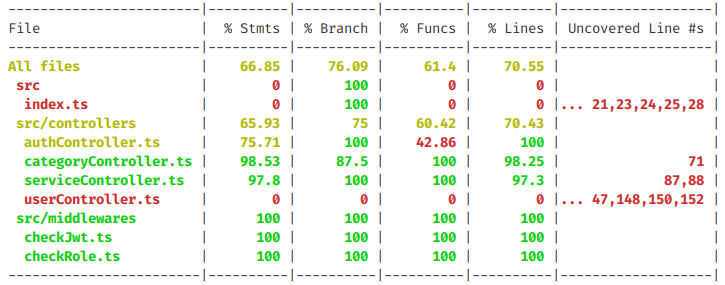
\includegraphics[width=\linewidth]{/test.png}
     \caption{The output of the code coverage reporter NYC}
     \label{fig:testResults}
 \end{figure}

We used a configuration to report files with 0-50\% coverage as red, 50-75\% as yellow and 75-100\% as green.
While this is a good indicator about how much of the code has been tested, it does not ensure that the tests are useful and correct.

To ensure this, we make use of formal reviews of both the code and tests.

\section{Integration testing}\label{sec:integrationTesting}
While unit testing is great for testing if a given module works in isolation, it is just as important to test if module A and B can work together as intended.
This is where integration testing comes in. 
Integration testing is an incremental process where an increasing amount of modules are put together and every time this happens the new and larger group is tested.
Integration testing is similar to unit testing, but it is a higher level of testing where we do not worry about the isolated functionality of the modules.
It is also common to use external libraries or module that are not necessarily developed by ourselves and it is therefor important to perform integration tests to make sure that the introduction of external module did not introduce any new bugs, or unexpected behavior. 

In this project, integration testing was been done in the API to verify that the external libraries added via the node package manager work as intended.
An example of an external library that was tested with integration testing is the \texttt{class-validator} package, where we give it a model that is intentionally wrong to see if it returns the data in the way we expect.
We can then continue on testing the controller where the validator is called, to see if it behaves as expected in case the class validator works.
This kind of testing can also be used for regression testing, as we will be made aware if the behavior of the validator changes due to the test failing.

\section{Formal review}
To ensure the quality of the code and the correctness of the tests, we made use of formal reviews.
A formal review is a process that belongs to the static white-box testing category.
A formal review contains four essential elements \cite{SoftwareTesting}:
\begin{itemize}\label{formalreview}
    \item Identify problems
    \item Follow rules
    \item Prepare
    \item Write a report
\end{itemize}
The goal of the review is to find problems or deficiencies in the software, with criticism directed at the design or the code itself.
Rules should be established regarding the process, such that they can be followed during a formal review.
An example of a rule could be defining the maximum amount of code to be reviewed at one time, or how many reviewers should examine the code.
Each participant in the review should be prepared for it, such that they can contribute.
Depending on the type of review, the participants could have different roles, and this should be known before the review begins, such that the roles can be actively fulfilled.
The review group should ultimately produce a report summarizing the results of the review, such that other developers can become aware of the results. 

\subsection{Our formal review process}
Initially when reviewing our code we would have two reviewers individually review the code and write comments and suggested changes. 
This would be done by creating a pull request (PR) to the develop branch and the author would then assign two reviewers.
When a review had been submitted by the reviewer, the author would go through the list of suggested changes to the code and fix the code or ask clarifying questions to the reviewer.
After two reviewers had accepted the PR it could be merged to the develop branch. 
\\\\
To further ensure that the quality of the code that is pushed to develop is of acceptable quality we use continuous integration (CI).
The CI ensures that the project is able to build without any errors, and that the unit tests succeed. 
That way we can be sure that the develop branch is never a broken build.
Additionally we use a linter that we can configure to test that the code follows some rules and coding standards. 
We also make the CI run the linter, and if the code does not follow the standards set it will fail to built.
\begin{figure}[H]
    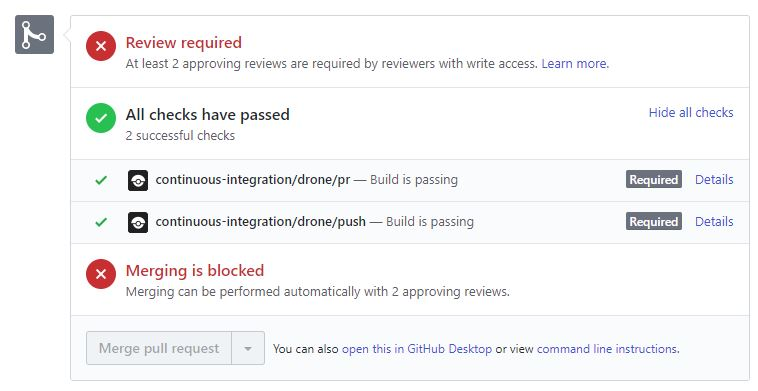
\includegraphics[width=\linewidth]{/ci.JPG}
    \caption{The CI has to be able to build for a PR to be merged}
    \label{fig:continous-integration}
\end{figure}
\noindent
During the later stages of the project we decided to change our approach to formal reviews.
Rather than have two developers individually review a PR, we strove to have the developers get together for the review.
This would ensure more discussions arose based on the PR, and increase the overall quality of the review.
\\\\
In terms of the four essential elements defined in \autoref{formalreview}, our process achieves these elements.
We did not directly write a report, as this element is mostly necessary for larger systems developed by larger teams.
Instead, the results of our reviews were made available through comments and suggestions to the PRs, such that other developers could access them.
\begin{figure}[H]
    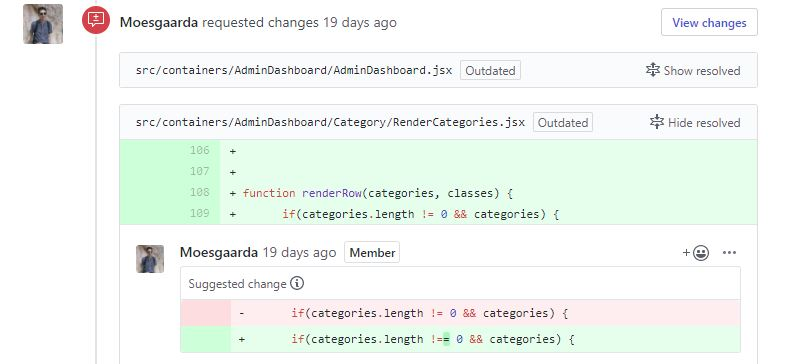
\includegraphics[width=\linewidth]{/commentonpr.JPG}
    \caption{An example of a comment on a PR}
    \label{fig:comment-on-pr}
\end{figure}

\section{Mutation testing}
Even with a code coverage of 100\%, the traditional test coverage measures only show how much of the code is executed by the tests, and not whether the tests are able to detect faults in the code \cite{pitest}.
This means that it is possible to get a full line, statement, and branch coverage by simply executing the code without any useful assertions in the test suite.
One way to combat this problem is with the use of mutation testing.
The idea behind mutation testing is to run some automated software (the mutation testing system), which will generate mutants by modifying minor parts of the system such as replacing a less than check with a greater than check.
The objective is to have a test suite that \textit{kills} the mutants by revealing that the mutant behavior differs from the original program \cite{mutationtesting}.

Mutation testing can be split into two categories: strong and weak mutations.
In strong mutation, we are only interested in the external observation of the code, meaning that the produced output of a given function is different when the mutation is introduced \cite{mutationtesting}.
These mutants can be hard to kill, since the effect of the mutant can be lost before the program terminates.
To be able to do a deeper check, we introduce weak mutation, where we define a mutant as killed if it leads to different results after \textit{some} execution, rather than after all code has finished executing.
Weak mutation testing is usually preferable to strong mutation testing in safety-critical systems, since it will be able to find more potential bugs, but with the tradeoff that execution time of the mutation analysis will increase.

After running the mutation test, the framework will generate a mutation score based on the percentage of mutants killed.
This can now be used to improve the test suite, by creating new test cases until all mutants can be killed.

\section{Usability testing}
Opposed to the previously mentioned tests, usability testing is not directly focused on the functionality and structure of the code, but rather how easy the system is to use by real users.
Even though the system may seem exceedingly simply to use by the developers, this is rarely the case for the actual users.
To increase the usability of the system during the development, the development team can make use of the personas defined in \autoref{sec:personas} during the formal review.
The reviewers can subjectively evaluate the design choices made against the personas and try to conclude whether all the personas would be able to understand the system.

However, this does not solve the problem of the reviewers knowing how the system works, and can easily navigate through it due to their deep understanding of the system.

Instead, it will be beneficial to conduct usability testing, where the testers try out the system under observation.
The testers, in this case, are usually either potential users of the system, or other employees who have not been a part of developing the software, to get more reliable results \cite{SoftwareTesting}.
\\\\
With usability testing, it is possible to get feedback on more subjective parts of the system, such as the user interface and whether the errors displayed to the user are useful and understandable without having a degree in software engineering \cite{SoftwareTesting}.

When conducting usability tests, a set of pre-defined tasks are given to the testers one at a time.
These tests should aim to resemble how actual users would use the system, to observe where they struggle to understand how the system works.

\subsection{Our usability tests}
To get feedback on the subjective parts of the system, we conducted usability tests.
The tests that the users performed can be found in \autoref{app:usability}.

\subsubsection{Comparison of the tests}
\autoref{tab:usabilitytest} shows the different testers and the time it took for them to perform the tasks defined.
The tester called Mikkel encountered some issues with logging in.
This was caused by some issues related to the test setup, and resulted in the time spent on the first few assignments not being indicative of the actual time it would take.
While the time was invalid, he still completed the assignments, looking for design deficiencies.
\begin{table}[]
    \begin{tabular}{|l|l|l|l|l|}
    \hline
                                            & Mikkel     & Melanie      & Martin           & Robin               \\ \hline
    Create user                             & N/A        & 1 min 31 sec & 1 min 24 sec     & 1 minute 11 seconds \\ \hline
    Log in                                  & N/A        & 10 seconds   & 34 seconds       & 18 seconds          \\ \hline
    Change language                         & N/A        & 15 seconds   & 14 seconds       & 12 seconds          \\ \hline
    Find "Butterfly"                        & N/A        & 13 seconds   & 12 seconds       & 10 seconds          \\ \hline
    Find other services by "Mathias Møller" & N/A        & 12 seconds   & 1 min 31 seconds & 13 seconds          \\ \hline
    Delete user                             & N/A        & 20 seconds   & 21 seconds       & 22 seconds          \\ \hline
    Login as admin                          & N/A        & 20 seconds   & 22 seconds       & 18 seconds          \\ \hline
    Create a service                        & 21 seconds & 38 seconds   & 45 seconds       & 30 seconds          \\ \hline
    Rate specific service                   & 10 seconds & 19 seconds   & 20 seconds       & 21 seconds          \\ \hline
    Log out                                 & 5 seconds  & 10 seconds   & 4 seconds        & 5 seconds           \\ \hline
    \end{tabular}
    \caption{A comparison of the time it took to perform the different tasks}
    \label{tab:usabilitytest}
\end{table}
Creating a user consistently took the longest amount of time.
As can be seen, for all applicable tester, it took longer than 1 minute.
The reason for this is that when creating a user, more input is required than many other parts of the system.
The testers encountered an issue with their passwords, as the restrictions put on this made them have to redo this.
The password requires at least 8 characters, with one number and one capital character.
Another consistent issue was the design of choosing a language when creating a user.
The user has to choose the languages they are capable of speaking, such that, if they were to become tutors and create a service, prospective learners would know in which languages the service could be provided.
During the test it was implemented as a dropdown in which users could select multiple languages at a time.
This turned out to be unintuitive, as they were unsure whether or not they had actually chosen a language after selecting one.
This led to some of them repeatedly clicking the same language multiple times, selecting and deselecting it.
A possible fix for these issues could be to close the dropdown once a language has been chosen, but this might not communicate that the user is capable of selecting multiple languages.
\\\\
The assignment to find other services by a certain tutor had the largest deviation in terms of time spent.
Two of the testers spent respectively 12 and 13 seconds, while the third spent a full minute and 31 seconds to complete the task.
The reason for this deviation is that the tester was confused what exactly he was supposed to do.
Once he figured it out, he felt it was not immediately obvious where to go.
Finally, he attempted to search for the tutor, which ended in him encountering a bug in which the search functionality did not work.
This bug has since been fixed such that users can search for the name of a tutor.
\\\\
One of the testers commented on the icons used in the system, saying some of them might not be as intuitive as intended.
This tester was confused with the log in button, thinking it looked like a log out button instead.
Generally, the assignments felt easy to complete for the testers.
Outside of the two discussions above, the assignments were completed quickly, and the testers spent around the same amount of time on all of them.
This, along with the lack of problems caused by the design during testing could indicate that, generally, the design of the system is fairly intuitive, while some of the icons could be a bit unintuitive. 



\chapter{Discussion}

\section{Reflections on our process}
In \autoref{sec:our-process} we described our process and the things that we used from Scrum.
In this section, we reflect on our process, and how it changed throughout the semester as well as what we would change for our future projects.

\subsubsection{Scrum}
Our Scrum inspired process worked well with sprints, sprint planning, sprint backlog, product owner, Scrum Master, planning poker, product backlog and product increment.
We took turns on having the role as PO and Scrum Master.
The PO/Scrum Master had the task of planning the next product backlog and add a DoD (definition of done) onto every task in the product backlog.
This person also had the responsibility to send material to the supervisor, book a conference room and responsible for the planning poker.
The sprint backlog and product backlog can be seen on \autoref{fig:trello-kanban}. 
This is an kanban board on Trello we use to give an overview of how far people are with their tasks.
The leftmost column is the product backlog, the next four column are the sprint backlog.
These are split into \textit{Sprint Backlog}, \textit{In progress}, \textit{In review} and \textit{Done}.

\begin{figure}[H]
    \centering
    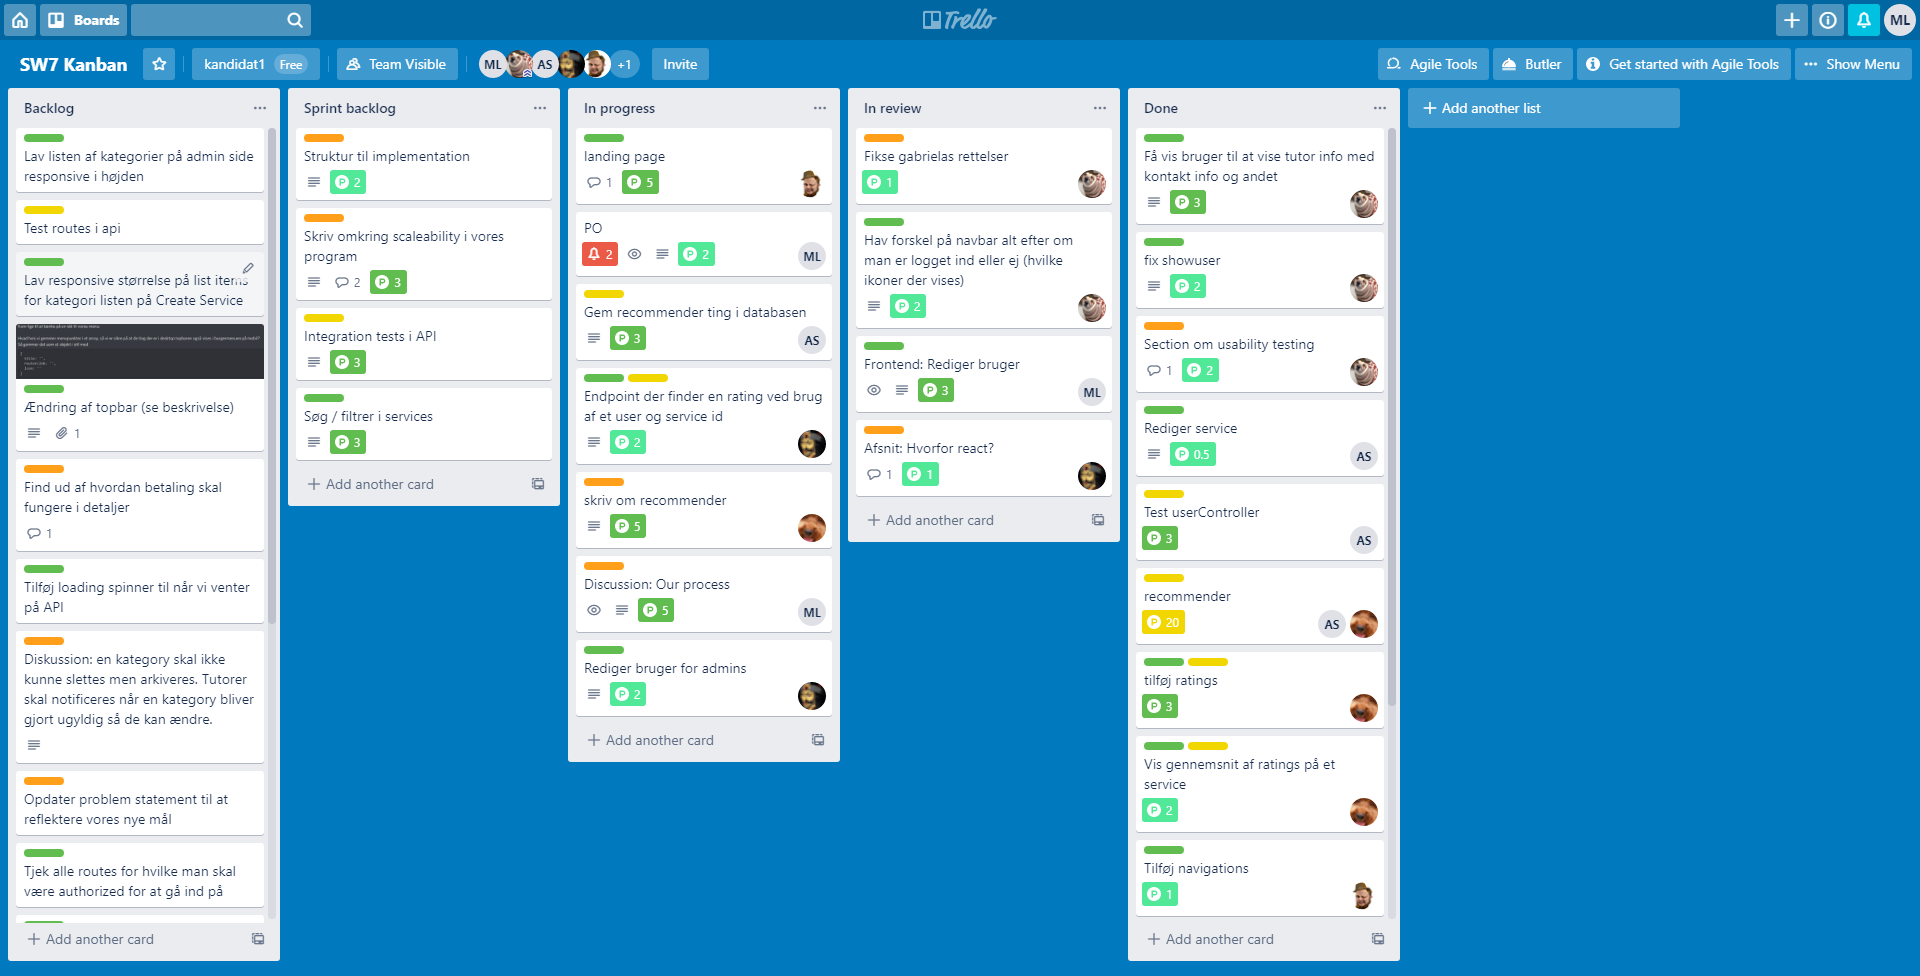
\includegraphics[width=0.8\linewidth]{figures/trellopicture.PNG}
    \caption{Our kanban board for the product and sprint backlog on Trello}
    \label{fig:trello-kanban}
\end{figure}
\noindent
When we conducted the sprint planning, we would use planning poker to estimate how many story points each task in the proposed sprint backlog should have.
The persons with the highest and lowest story points would discuss the reasoning behind it.
The story points were often very different if there were ambiguities, and people understood the tasks differently.
This gave everyone the same understanding on how the given tasks should be solved and eliminate most ambiguities. 
\\
However, in the middle of the project when we started to develop the application and learning \textit{React}, it started to become less systematic.
This was often due to it being difficult to estimate how long each task would take to solve.
When we got more familiar with \textit{React} we were able to estimate how much the tasks took, and it got more systematic again.
\\\\
We also stopped conducting the retrospective meetings.
The Scrum Masters stopped enforcing the retrospective meetings so they started fading out.
These meetings could have helped making the project more structured as we could have discussed the problems that we faced and the reasons why we did not complete our tasks in time.

\subsubsection{Formal reviews}
The formal reviews was something that we changed in the middle of the semester, so that two people had to review a pull request together.
Previously people would review a pull request individually.
Formal reviews were described in \autoref{sec:formal-reviews}.
The first hour of every workday was spent on reviewing pull requests.
\\\\
This increased the quality of the pull requests, as more errors were caught when two people had to debate the code.
This is however more time consuming and more difficult to plan.
If two people are in process of reviewing a pull request another person can be waiting for them to finish if they are assigned a pull request with one of them. 
Then when a pull request have been reviewed and if changes are requested, then these people have to come back to review the changes.
To make this more organized a we created a PR spreadsheet to give an better overview of which pull requests you are assigned to, and who are currently requested to do many or few reviews.
This can be seen on \autoref{fig:formal-reviews}.
\begin{figure}[H]
    \centering
    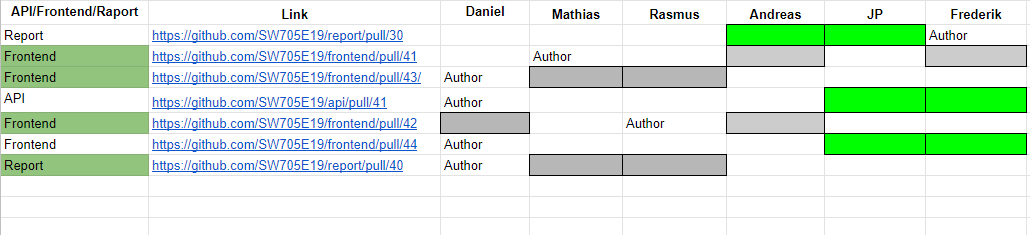
\includegraphics[width=\linewidth]{figures/formal-reviews.PNG}
    \caption{Pull request assignment sheet.}
    \label{fig:formal-reviews}
\end{figure}

\subsubsection{Working from home}
Unlike other semesters, we were not assigned a group room this semester.
This resulted in us working from home most days in the week, because we thought this would be easier and as productive as if we met at the university.
One of the cons of working from home is that it is more difficult to get help from the other group members and this can lead people to get stuck on tasks.
After a few weeks we realized that it would be better if we had one workday together every week.
This was really beneficial as the more experienced React developers were able to help other members that were less experienced.
It was also easier to conduct a sprint planning when we met in person.

\subsubsection{Supervisor meetings}
The day before the supervisor meeting we sent the report, a reading guide and an agenda for the meeting.
Our supervisor gave feedback on the material that we sent to her and during the meeting we presented the things that we had done the previous week.
These meetings have been longer than the meetings we had previously experienced in last semesters, but this also resulted in better feedback, as the questions she asked made us reflect on certain choices we had made.

\subsubsection{What we would do differently}
One of the problems that we faced was that people could get stuck on tasks.
For future projects we would try to be more aware of where people are in the process, so that it would be easier to help them with solving their tasks.
One of the solutions to this could be daily standups, so that we are aware of where people are with their tasks, and which once they have not completed.

Another solution could be to have more workdays at the university, so that people have an easier time getting help from one another.
It is especially important in the beginning of the semester when there are still a lot of ambiguities and uncertainties with the project.  

We would also like to hold the retrospective meeting so that we had to reflect on the previous week and correcting the problems that we faced.

When adding tasks to the product backlog it should also be a requirement to add a DoD, as we multiple times were unable to recognize what needed to be done from just the title.

\section{Future work}
The tasks for future work focuses on completing the tasks in our MoSCoW.

There are 5 tasks that we would like to implement.

\begin{itemize}
    \item Upload and view material
    \item Messaging system
    \item Calendar system
    \item On-site payment
    \item Booking a tutor
\end{itemize}

\textit{Upload and view material}:
We would like the option for 
\include{sections/conclusion/conclusion}
\chapter{Appendix}

\section{Load testing results}
\subsection{1 instance}
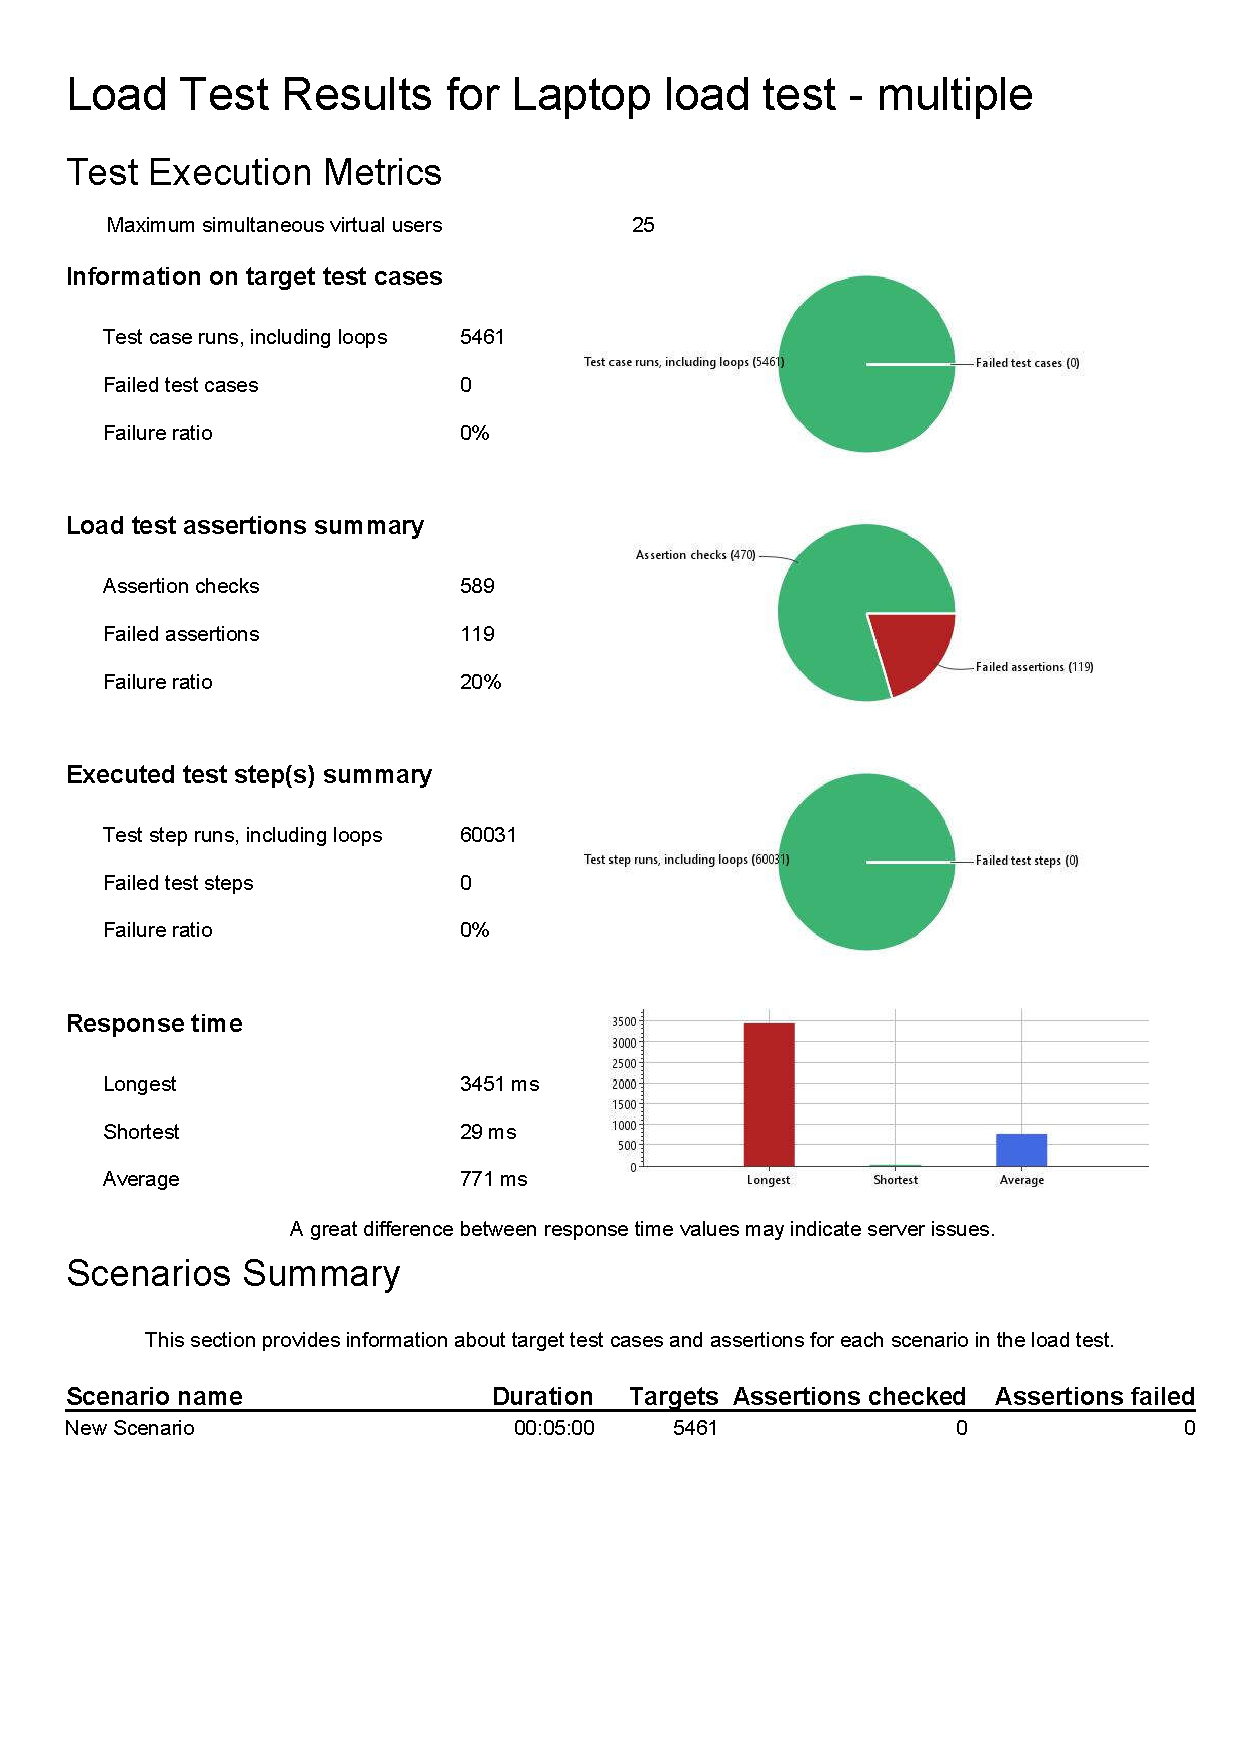
\includepdf{sections/appendix/1_instance-s12.pdf}
\subsection{4 instances}
\includepdf{sections/appendix/4.1_instance23.pdf}
\subsection{8 instances}
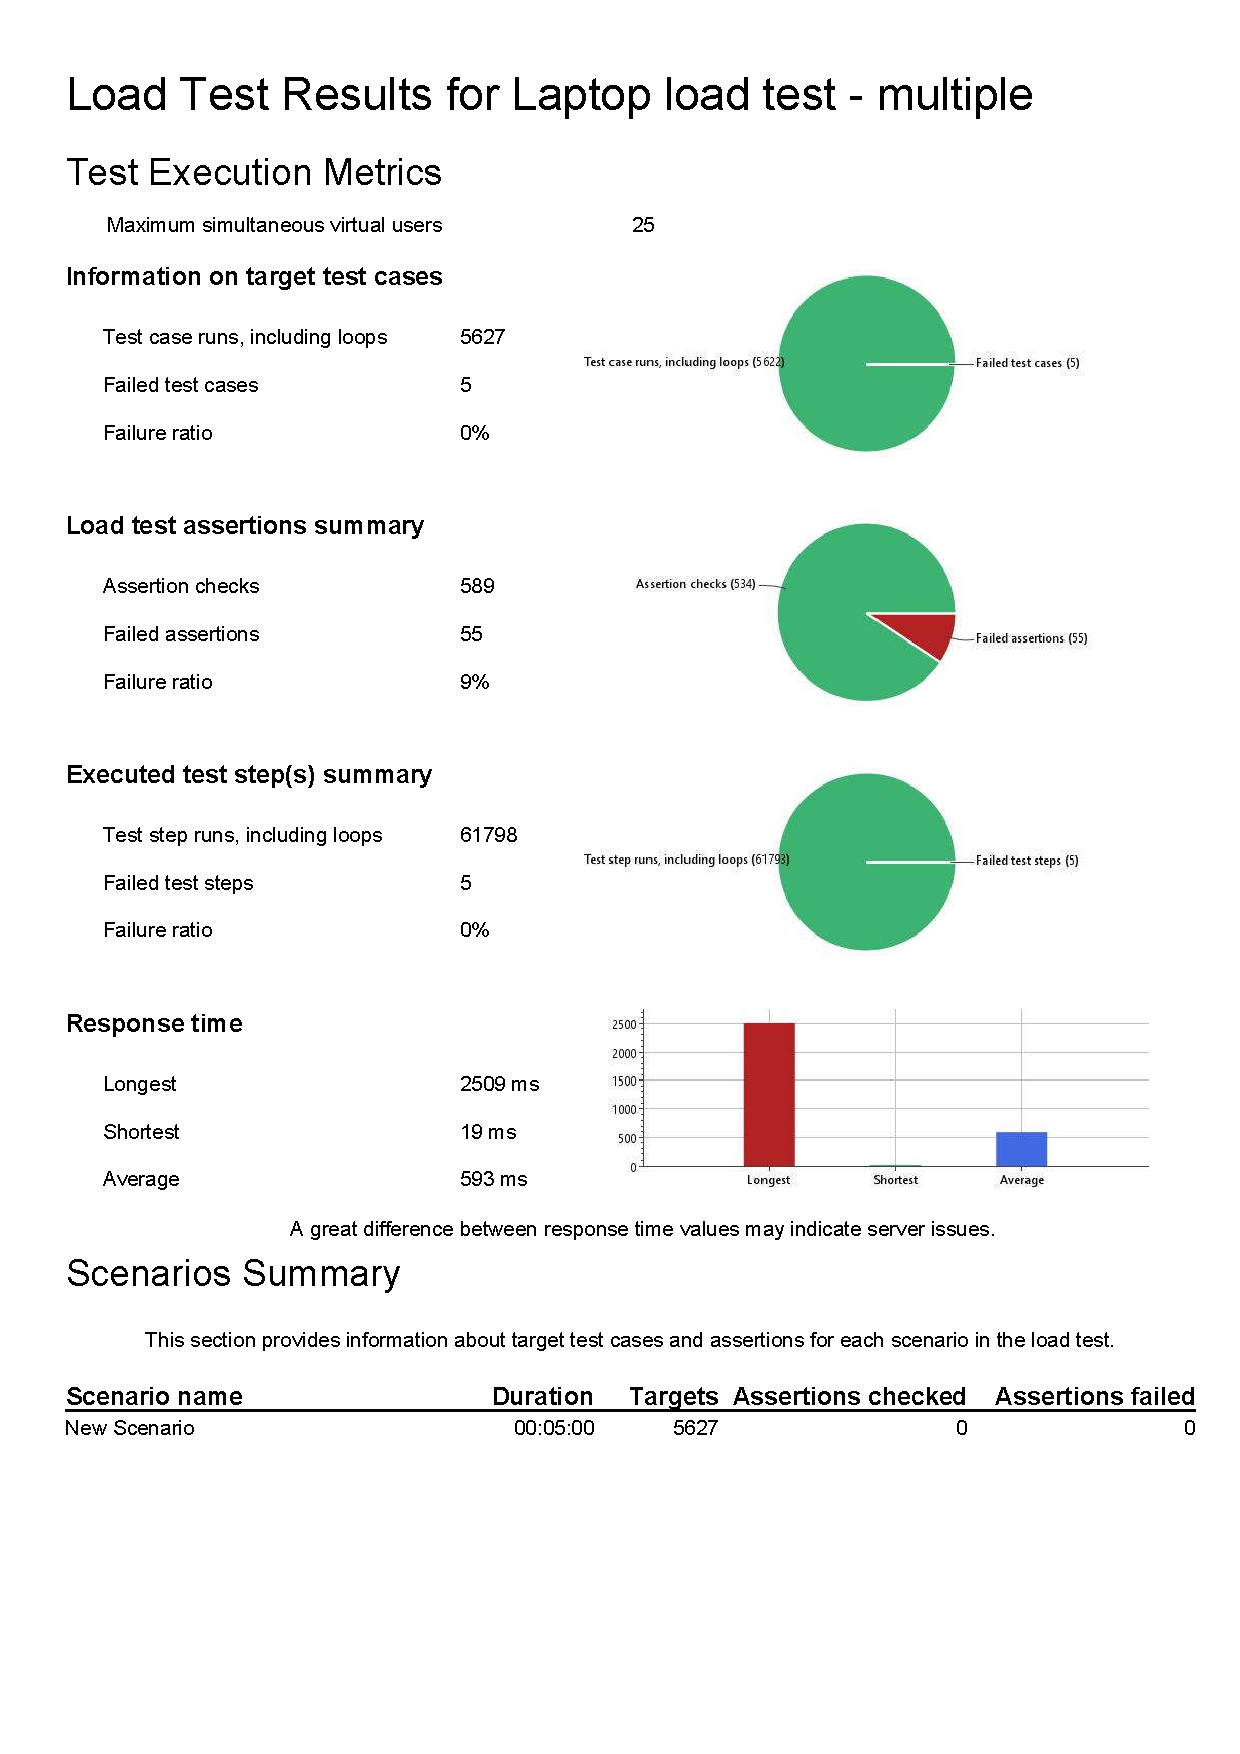
\includepdf{sections/appendix/8_Instance23.pdf}
\subsection{16 instances}
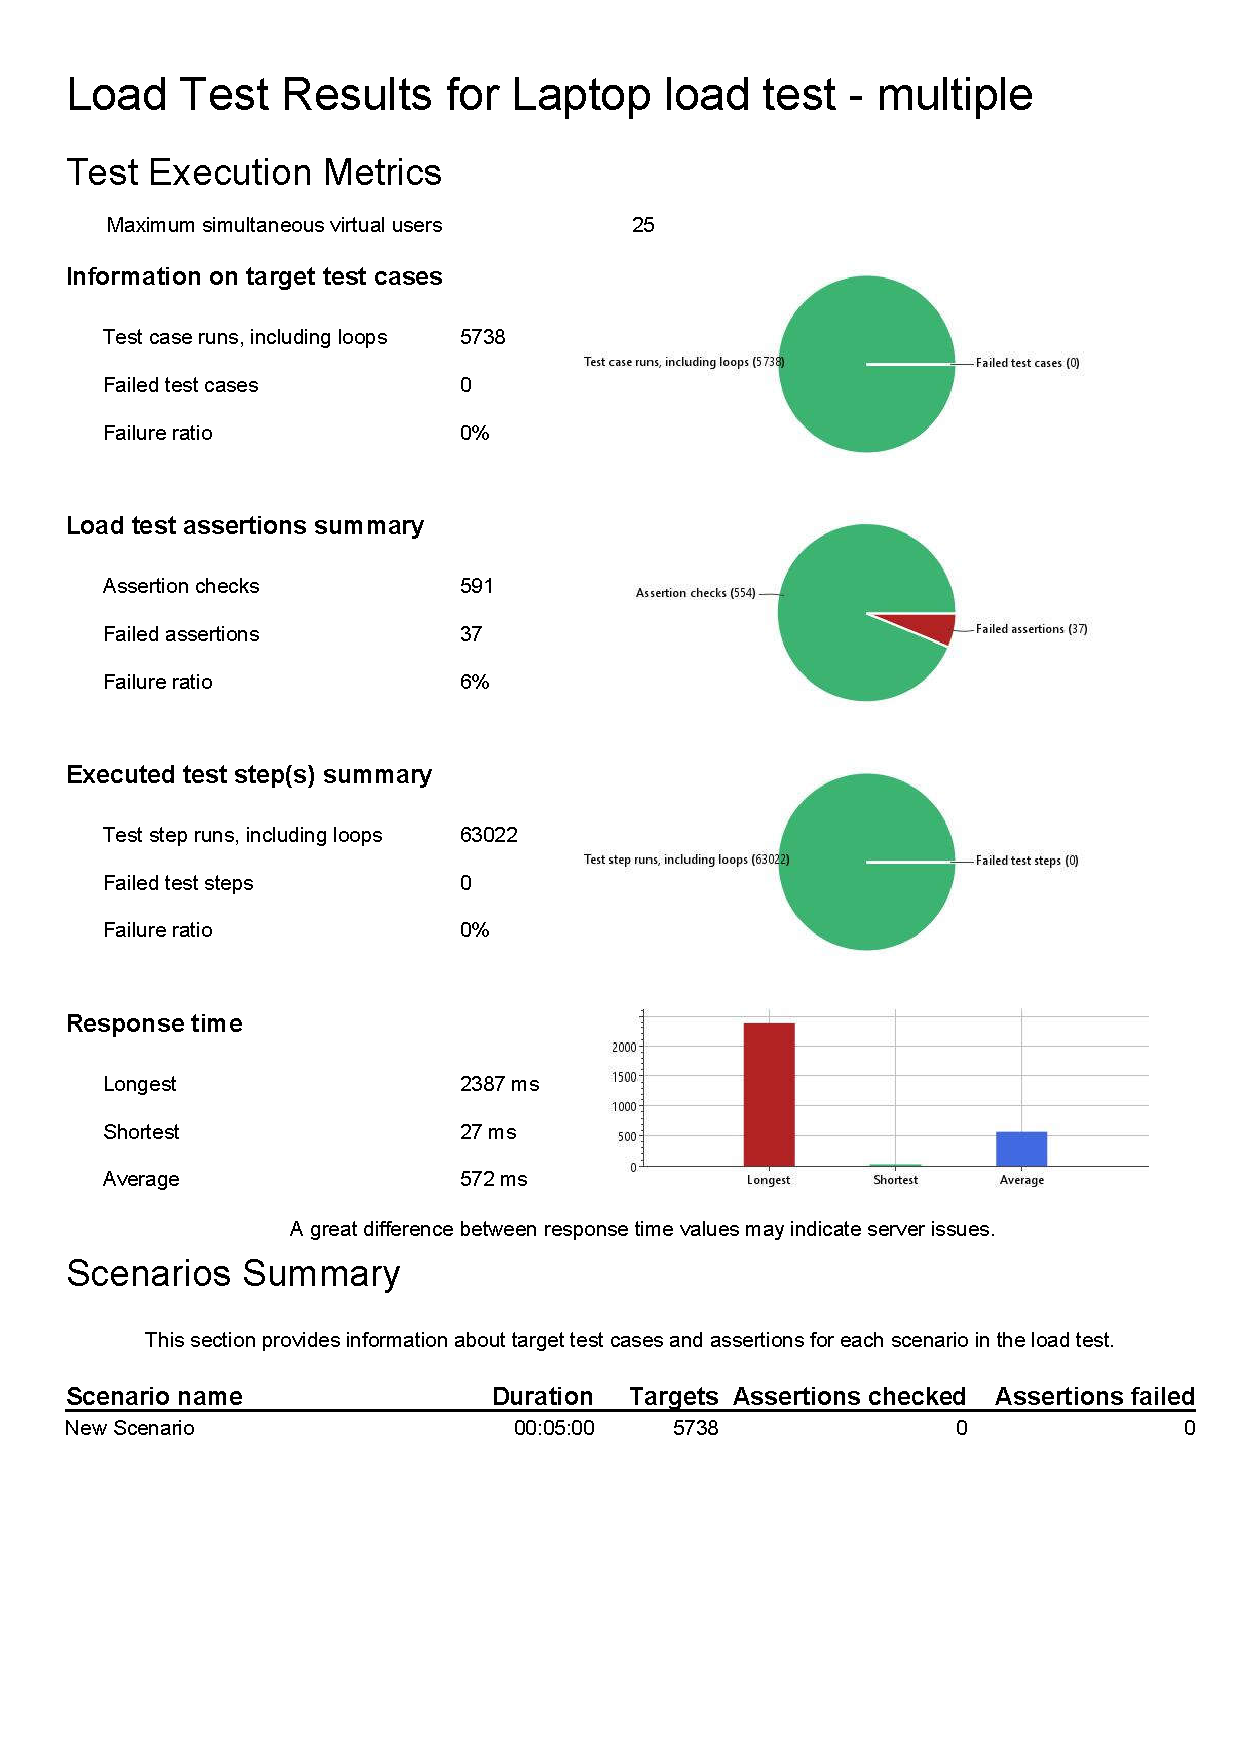
\includepdf{sections/appendix/16_instance23.pdf}
\subsection{32 instances}
\includepdf{sections/appendix/32_instance32.pdf}

\printbibliography[heading=bibintoc]
\label{bib:mybiblio}
\listoffigures
\listoftables
\lstlistoflistings

%\listoftodos
%\todo{Todo regler:}
%\todo[color=purple]{Purple = Skal diskuteres}
%\todo[color=green]{Green = Er skrevet færdigt, men mangler at blive læst.}
%\todo[color=blue]{Blue = Skal skives, men vi har ikke haft om det endnu.}
%\todo[color=red]{Red = Ændret, men ikke færdigt.}
%\todo[color=white]{White = Kommentar}
%\todo[color=pink]{Pink = T. Hansen er i gang.}
%\todo[color=yellow]{Yellow = R. Eduardsen er i gang.}
%\todo[color=gray]{Gray = J.P. Tróndarson er i gang.}
%\todo[color=cyan]{Cyan = D. Andersen er i gang.}
%\todo[color=brown]{Brown = F. Schrøder er i gang.}
%\todo[color=magenta]{Magenta = A. Stenshøj er i gang.}
\end{document}
